% Chapter 1

\chapter{Introducción general} % Main chapter title

\label{Chapter1} % For referencing the chapter elsewhere, use \ref{Chapter1} 
\label{IntroGeneral}

%----------------------------------------------------------------------------------------

% Define some commands to keep the formatting separated from the content 
\newcommand{\keyword}[1]{\textbf{#1}}
\newcommand{\tabhead}[1]{\textbf{#1}}
\newcommand{\code}[1]{\texttt{#1}}
\newcommand{\file}[1]{\texttt{\bfseries#1}}
\newcommand{\option}[1]{\texttt{\itshape#1}}
\newcommand{\grados}{$^{\circ}$}

%----------------------------------------------------------------------------------------

%\section{Introducción}
En el presente capitulo se expone el principio de funcionamiento de las maquinas CNC, sus componentes principales, su interconeccion y uso. Luego se explica la problematica de la alineacion de piezas 2D y algunas soluciones.
%----------------------------------------------------------------------------------------
\section{Descripcion del problema}



\subsection{Una introducción (no tan corta) a \LaTeX{}}

Si sos nuevo en \LaTeX{}, hay un muy buen libro electrónico - disponible gratuitamente en Internet como un archivo PDF - llamado, \enquote{A (not so short) Introduction to \LaTeX{}}. El título del libro es generalmente acortado a simplemente \emph{lshort}. Puede descargar la versión más reciente en inglés (ya que se actualiza de vez en cuando) desde aquí:
\url{http://www.ctan.org/tex-archive/info/lshort/english/lshort.pdf}

Se puede encontrar la versión en español en la lista en esta página: \url{http://www.ctan.org/tex-archive/info/lshort/}

\subsubsection{Una subsubsección}

Acá tiene un ejemplo de una ``subsubsección'' que es el cuarto nivel de ordenamiento del texto, después de capítulo, sección y subsección.  Como se puede ver, las subsubsecciones no van numeradas en el cuerpo del documento ni en el índice.  El formato está definido por la plantilla y no debe ser modificado.

\subsection{Guía matemática rápida para \LaTeX{}}

Si estás escribiendo un documento con mucho contenido matemático, entonces es posible que desees leer el documento de la AMS (American Mathematical Society) llamado, \enquote{A Short Math Guide for \LaTeX{}}. Se puede encontrar en línea en el siguiente link: \url{http://www.ams.org/tex/amslatex.html} en la sección \enquote{Additional Documentation} hacia la parte inferior de la página.


%----------------------------------------------------------------------------------------

\section{Utilizando esta plantilla}

Si estás familiarizado con \LaTeX{}, entonces podés explorar la estructura de directorios de esta plantilla y proceder a personalizarla agregando tu información en el bloque \emph{INFORMACIÓN DE LA PORTADA} en el archivo \file{memoria.tex}.  

Se puede continuar luego modificando el resto de los archivos siguiendo los lineamientos que se describen en la sección \ref{sec:FillingFile} en la página \pageref{sec:FillingFile}.

Debés asegurarte de leer el capítulo \ref{Chapter2} acerca de las convenciones utilizadas para las Memoria de los Trabajos Finales de la \degreename.

Si sos nuevo en \LaTeX{}, se recomienda que continúes leyendo el documento ya que contiene información básica para aprovechar el potencial de esta herramienta.


%----------------------------------------------------------------------------------------

\section{Qué incluye esta plantilla}

\subsection{Carpetas}

Esta plantilla se distribuye como una único archivo .zip que se puede descomprimir en varios archivos y carpetas. Asimismo, se puede consultar el repositorio git para obtener la última versión de los archivos, \url{https://github.com/patriciobos/Plantilla-CESE.git}. Los nombres de las carpetas son, o pretender ser, auto-explicativos.

\keyword{Appendices} -- Esta es la carpeta donde se deben poner los apéndices. Cada apéndice debe ir en su propio archivo \file{.tex}. Se incluye un ejemplo y una plantilla en la carpeta.

\keyword{Chapters} -- Esta es la carpeta donde se deben poner los capítulos de la memoria. Cada capítulo debe ir un su propio archivo \file{.tex} por separado.  Se ofrece por defecto, la siguiente estructura de capítulos y se recomienda su utilización dentro de lo posible:

\begin{itemize}
\item Capítulo 1: Introducción general	
\item Capítulo 2: Introducción específica
\item Capítulo 3: Diseño e implementación
\item Capítulo 4: Ensayos y resultados
\item Capítulo 5: Conclusiones

\end{itemize}

Esta estructura de capítulos es la que se recomienda para las memorias de la especialización.

\keyword{Figures} -- Esta carpeta contiene todas las figuras de la memoria.  Estas son las versiones finales de las imágenes que van a ser incluidas en la memoria.  Pueden ser imágenes en formato \textit{raster}\footnote{\url{https://en.wikipedia.org/wiki/Raster_graphics}} como \file{.png}, \file{.jpg} o en formato vectoriales\footnote{\url{https://en.wikipedia.org/wiki/Vector_graphics}} como \file{.pdf}, \file{.ps}.  Se debe notar que utilizar imágenes vectoriales disminuye notablemente el peso del documento final y acelera el tiempo de compilación por lo que es recomendable su utilización siempre que sea posible.

\subsection{Archivos}

También están incluidos varios archivos, la mayoría de ellos son de texto plano y se puede ver su contenido en un editor de texto. Después de la compilación inicial, se verá que más archivos auxiliares son creados por \ LaTeX{} o BibTeX, pero son de uso interno y no es necesario hacer nada en particular con ellos.  Toda la información necesaria para compilar el documento se encuentra en los archivos \file{.tex}, \file{.bib}, \file{.cls} y en las imágenes de la carpeta Figures.

\keyword{referencias.bib} - este es un archivo importante que contiene toda la información de referencias bibliográficas que se utilizarán para las citas en la memoria en conjunto con BibTeX. Usted puede escribir las entradas bibliográficas en forma manual, aunque existen también programas de gestión de referencias que facilitan la creación y gestión de las referencias y permiten exportarlas en formato BibTeX.  También hay disponibles sitios web como \url{books.google.com} que permiten obtener toda la información necesaria para una cita en formato BibTeX. Ver sección \ref{sec:biblio}

\keyword{MastersDoctoralThesis.cls} -- este es un archivo importante. Es el archivos con la clase que le informa a \LaTeX{} cómo debe dar formato a la memoria. El usuario de la plantilla no debería necesitar modificar nada de este archivo.

\keyword{memoria.pdf} -- esta es su memoria con una tipografía bellamente compuesta (en formato de archivo PDF) creado por \LaTeX{}. Se distribuye con la plantilla y después de compilar por primera vez sin hacer ningún cambio se debería obtener una versión idéntica a este documento.

\keyword{memoria.tex} -- este es un archivo importante. Este es el archivo que tiene que compilar \LaTeX{} para producir la memoria como un archivo PDF. Contiene un marco de trabajo y estructuras que le indican a \LaTeX{} cómo diagramar la memoria.  Está altamente comentado para que se pueda entender qué es lo que realiza cada línea de código y por qué está incluida en ese lugar.  En este archivo se debe completar la información personalizada de las primeras sección según se indica en la sección \ref{sec:FillingFile}.

Archivos que \emph{no} forman parte de la distribución de la plantilla pero que son generados por \LaTeX{} como archivos auxiliares necesarios para la producción de la memoria.pdf son:

\keyword{memoria.aux} -- este es un archivo auxiliar generado por \LaTeX{}, si se borra \LaTeX{} simplemente lo regenera cuando se compila el archivo principal \file{memoria.tex}.

\keyword{memoria.bbl} -- este es un archivo auxiliar generado por BibTeX, si se borra BibTeX simplemente lo regenera cuando se compila el archivo principal \file{memoria.tex}. Mientras que el archivo \file{.bib} contiene todas las referencias que hay, este archivo \file{.bbl} contine sólo las referencias que han sido citadas y se utiliza para la construcción de la bibiografía.

\keyword{memoria.blg} -- este es un archivo auxiliar generado por BibTeX, si se borra BibTeX simplemente lo regenera cuando se compila el archivo principal \file{memoria.tex}.

\keyword{memoria.lof} -- este es un archivo auxiliar generado por \LaTeX{}, si se borra \LaTeX{} simplemente lo regenera cuando se compila el archivo principal \file{memoria.tex}.  Le indica a \LaTeX{} cómo construir la sección \emph{Lista de Figuras}.
 
\keyword{memoria.log} --  este es un archivo auxiliar generado por \LaTeX{}, si se borra \LaTeX{} simplemente lo regenera cuando se compila el archivo principal \file{memoria.tex}. Contiene mensajes de \LaTeX{}. Si se reciben errores o advertencias durante la compilación, se guardan en este archivo \file{.log}.

\keyword{memoria.lot} -- este es un archivo auxiliar generado por \LaTeX{}, si se borra \LaTeX{} simplemente lo regenera cuando se compila el archivo principal \file{memoria.tex}.  Le indica a \LaTeX{} cómo construir la sección \emph{Lista de Tablas}.

\keyword{memoria.out} -- este es un archivo auxiliar generado por \LaTeX{}, si se borra \LaTeX{} simplemente lo regenera cuando se compila el archivo principal \file{memoria.tex}.

De esta larga lista de archivos, sólo aquellos con la extensión \file{.bib}, \file{.cls} y \file{.tex} son importantes.  Los otros archivos auxiliares pueden ser ignorados o borrados ya que \LaTeX{} y BibTeX los regenerarán durante la compilación.

%----------------------------------------------------------------------------------------

\section{Entorno de trabajo}

Ante de comenzar a editar la plantilla debemos tener un editor \LaTeX{} instalado en nuestra computadora.  En forma análoga a lo que sucede en lenguaje C, que se puede crear y editar código con casi cualquier editor, existen ciertos entornos de trabajo que nos pueden simplificar mucho la tarea.  En este sentido, se recomienda, sobre todo para los principiantes en \LaTeX{} la utilización de TexMaker, un programa gratuito y multi-plantaforma que está disponible tanto para windows como para sistemas GNU/linux.

La versión más reciente de TexMaker es la 4.5 y se puede descargar del siguiente link: \url{http://www.xm1math.net/texmaker/download.html}. Se puede consultar el manual de usuario en el siguiente link: \url{http://www.xm1math.net/texmaker/doc.html}.
 

\subsection{Paquetes adicionales}

Si bien durante el proceso de instalación de TexMaker, o cualquier otro editor que se haya elegido, se instalarán en el sistema los paquetes básicos necesarios para trabajar con \LaTeX{}, la plantilla de los trabajos de Especialización y Maestría requieren de paquete adicionales.

Se indican a continuación los comandos que se deben introducir en la consola de Ubuntu (ctrl + alt + t) para instalarlos:

\begin{lstlisting}[language=bash]
  $ sudo apt install texlive-lang-spanish texlive-science 
  $ sudo apt install texlive-bibtex-extra biber
  $ sudo apt install texlive texlive-fonts-recommended
  $ sudo apt install texlive-latex-extra
\end{lstlisting}


\subsection{Configurando TexMaker}


Una vez instalado el programa y los paquetes adicionales se debe abrir el archivo memoria.tex con el editor para ver una pantalla similar a la que se puede apreciar en la figura \ref{fig:texmaker}. 

\begin{figure}[h]
	\centering
	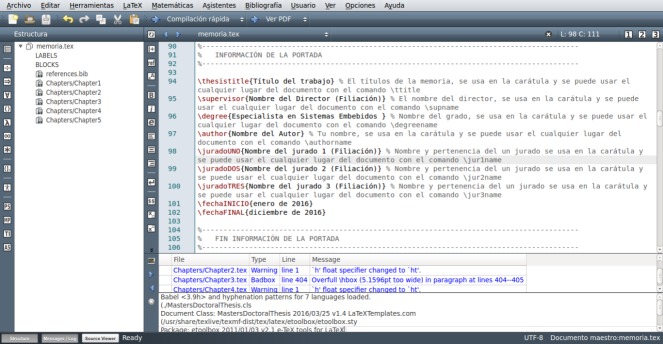
\includegraphics[width=\textwidth]{./Figures/texmaker.png}
	\caption{Entorno de trabajo de texMaker.}
	\label{fig:texmaker}
\end{figure}

Notar que existe una vista llamada Estructura a la izquierda de la interfaz que nos permite abrir desde dentro del programa los archivos individuales de los capítulos.  A la derecha se encuentra una vista con el archivo propiamente dicho para su edición. Hacia la parte inferior se encuentra una vista del log con información de los resultados de la compilación.  En esta última vista pueden aparecen advertencias o \textit{warning}, que normalmente pueden ser ignorados, y los errores que se indican en color rojo y deben resolverse para que se genere el PDF de salida.

Recordar que el archivo que se debe compilar con PDFLaTeX es \file{memoria.tex}, si se tratara de compilar alguno de los capítulos saldría un error.  Para salvar la molestia de tener que cambiar de archivo para compilar cada vez que se realice una modificación en un capítulo, se puede definir el archivo \file{memoria.tex} como ``documento maestro'' yendo al menú opciones -> ``definir documento actual como documento maestro'', lo que permite compilar con PDFLaTeX memoria.tex directamente desde cualquier archivo que se esté modificando . Se muestra esta opción en la figura \ref{fig:docMaestro}.

\begin{figure}[h]
	\centering
	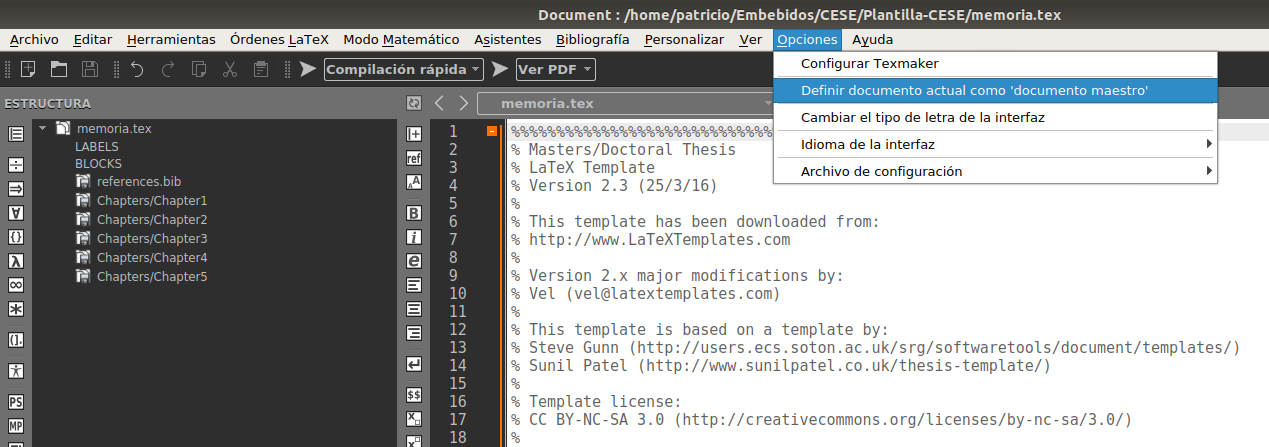
\includegraphics[width=\textwidth]{./Figures/docMaestro.png}
	\caption{Definir memoria.tex como documento maestro.}
	\label{fig:docMaestro}
\end{figure}

En el menú herramientas se encuentran las opciones de compilación.  Para producir un archivo PDF a partir de un archivo .tex se debe ejecutar PDFLaTeX (el shortcut es F6). Para incorporar nueva bibliografía se debe utilizar la opción BibTeX del mismo menú herramientas (el shortcut es F11).

Notar que para actualizar las tablas de contenidos se debe ejecutar PDFLaTeX dos veces.  Esto se debe a que es necesario actualizar algunos archivos auxiliares antes de obtener el resultado final.  En forma similar, para actualizar las referencias se debe ejecutar primero PDFLaTeX, después BibTeX y finalmente PDFLaTeX dos veces por idénticos motivos.

\section{Personalizando la plantilla, el archivo \file{memoria.tex}}
\label{sec:FillingFile}

Para personalizar la plantilla se debe incorporar la información propia en los distintos archivos \file{.tex}. 

Primero abrir \file{memoria.tex} con TexMaker (o el editor de su preferencia). Se debe ubicar dentro del archivo el bloque de código titulado \emph{INFORMACIÓN DE LA PORTADA} donde se deben incorporar los primeros datos personales con los que se construirá automáticamente la portada.


%----------------------------------------------------------------------------------------

\section{El código del archivo \file{memoria.tex} explicado}

El archivo \file{memoria.tex} contiene la estructura del documento y es el archivo de mayor jerarquía de la memoria.  Podría ser equiparable a la función \emph{main()} de un programa en C, o mejor dicho al archivo fuente .c donde se encuentra definida la función main().

La estructura básica de cualquier documento de \LaTeX{} comienza con la definición de clase del documento, es seguida por un preámbulo donde se pueden agregar funcionalidades con el uso de \texttt{paquetes} (equiparables a bibliotecas de C), y finalmente, termina con el cuerpo del documento, donde irá el contenido de la memoria.

\lstset{%
  basicstyle=\small\ttfamily,
  language=[LaTeX]{TeX}
}

\begin{lstlisting}
\documentclass{article}  <- Definicion de clase
\usepackage{listings}	 <- Preambulo

\begin{document}	 <- Comienzo del contenido propio 
	Hello world!
\end{document}
\end{lstlisting}


El archivo \file{memoria.tex} se encuentra densamente comentado para explicar qué páginas, secciones y elementos de formato está creando el código \LaTeX{} en cada línea. El código está dividido en bloques con nombres en mayúsculas para que resulte evidente qué es lo que hace esa porción de código en particular. Inicialmente puede parecer que hay mucho código \LaTeX{}, pero es principalmente código para dar formato a la memoria por lo que no requiere intervención del usuario de la plantilla.  Sí se deben personalizar con su información los bloques indicados como:

\begin{itemize}
	\item Informacion de la memoria
	\item Resumen
	\item Agradecimientos
	\item Dedicatoria
\end{itemize}

El índice de contenidos, las listas de figura de tablas se generan en forma automática y no requieren intervención ni edición manual por parte del usuario de la plantilla. 

En la parte final del documento se encuentran los capítulos y los apéndices.  Por defecto se incluyen los 5 capítulos propuestos que se encuentran en la carpeta /Chapters. Cada capítulo se debe escribir en un archivo .tex separado y se debe poner en la carpeta \emph{Chapters} con el nombre \file{Chapter1}, \file{Chapter2}, etc\ldots El código para incluir capítulos desde archivos externos se muestra a continuación.

\begin{verbatim}
	% Chapter 1 
\chapter{Introducción general} % Main chapter title

En el presente capítulo se introducen ejemplos de uso de las máquinas de control numérico y las dificultades que presentan para alinearse con las piezas a mecanizar. Luego se comparan soluciones de otros fabricantes y finalmente se comenta acerca de la motivación, el alcance y los objetivos de la propia.

\label{Chapter1} % For referencing the chapter elsewhere, use \ref{Chapter1} 
\label{IntroGeneral}

%----------------------------------------------------------------------------------------
\section{Historia y principio de funcionamiento}

Hacia finales de la década del '40, el mecánico inventor Jhon Parsons\footnote\jhonparsonwiki retratado en la figura \ref{fig:parsons_A}, logró motorizar una agujereadora de banco de precisión y la automatizó mediante el uso de una cinta perforada, figura \ref{fig:parsons_B}.\\
A este invento se lo considera la primera máquina de control numérico o NC por sus siglas en inglés (\textit{numerical control}).
\subfigab
         {0.37}{parsons_face}{Fotografia de Jhon T. Parsons, considerado en la industria como el inventor de las máquinas NC.}{fig:parsons_A}
         {0.6}{parsons_machine}{Una de las primeras máquinas de la industria consideradas de control numérico NC.\\ \vphantom{1}}{fig:parsons_B}
         {Jhon Parsons, el inventor de las máquinas de control numérico junto a una de sus máquinas.}
         {fig:parsons}
\par
Luego de varias décadas, con el surgimiento de las computadoras, se reemplazaron las cintas perforadas por software, dando lugar a las máquinas de control numérico computarizado o CNC por sus siglas en inglés \textit{(computer numerical control)}.
\\
A pesar del paso del tiempo y los avances tecnológicos, los bloques constitutivos de una máquina CNC siguen siendo los mismos que se muestran en la figura \ref{fig:cnc_main_blocks}.
\subfiga {1}
         {cnc_main_blocks.pdf}
         {Los tres bloques básicos de una máquina CNC.}
         {fig:cnc_main_blocks}

\subsection{Programa de movimientos}
   El programa de movimientos consiste en una serie de instrucciones necesarias para obtener una determinada pieza y se escribe en un un lenguaje conocido como GCode\citep{WEBSITE:gcode_wiki}.\par
   Este lenguaje fue creado por el Instituto tecnológico de Masachussets en la década del '50 y especificado en el documento NIST-RS274-D \citep{rs274}.\par
Originalmente los ingenieros de mecanizado lo escribían manualmente en una planilla y luego, mediante una máquina de mecanografía, se transcribía a una cinta perforada que sería interpretada por el controlador de movimientos.\par
Se pueden ver algunas fotos de este primigenio proceso en la figura \ref{fig:programacion_cnc_primigenia}.
\subfigtwotwo
          {0.46}{cad_cam_primigenio1} {Ingeniero escribiendo en papel la lista de operaciones para mecanizar una pieza en lenguaje GCode.}
          {0.5}{cad_cam_primigenio2} {Operadora transcribiendo la lista de operaciones del formato papel a un rollo de cinta multiperforada.}
          {0.46}{cad_cam_primigenio3} {Lector de cinta multiperforada que controla los movimientos de la máquina.}
          {0.5}{cad_cam_primigenio4} {Operador trabajando con una de las primeras fresadoras por control numerico.}
          {Secuencia de pasos para operar una máquina NC primigenia.}
          {fig:programacion_cnc_primigenia}


          En el presente se diseña la pieza en tres dimensiones con la ayuda de software de diseño asistido por computadora CAD  (\textit{computer aided design}).\\
          Algunos software de CAD reconocidos se listan a continuación:
          \begin{itemize}
             \item{FreeCAD}
             \item{Blender}
             \item{Rhinoceros}
             \item{AutoCAD}
             \item{SolidWorks}
          \end{itemize}
   El archivo de salida del CAD se procesa con un software de manufactura asistida por computadora CAM (\textit{computer aided manufacturing}) en donde el diseñador puede configurar los métodos y estrategias de mecanizado.\par
          Algunos software de CAM reconocidos se listan a continuación:
          \begin{itemize}
             \item{RhinoCAM}
             \item{Blender CAM}
             \item{FreeMILL}
             \item{Aspire}
             \item{Mastercam}
          \end{itemize}

   El resultado final es un archivo de texto en lenguaje GCode que se almacena digitalmente y que será procesado por el controlador.\par
          Esta secuencia es conocida como diseño CAD/CAM y se muestra en la figura \ref{fig:programacion_cnc_actual}
\subfigtwotwo 
            {0.48 }{cad_cnc_cuadrado}{Se diseña la pieza en 3D en un software CAD.\\ \vphantom{1}}
            {0.48 }{cam_cnc_cuadrado}{Se diseña la estrategia de mecanizado y opcionalmente se simula el proceso en un software CAM.}
            {0.48 }{gcode_cnc_cuadrado}{Se exporta desde el CAM un archivo en lenguaje GCode con las instrucciones de máquina que leerá el controlador.}
            {0.40 }{portada_mach3}{El sofware del controlador genera las señales que mueven el CNC y ejecutan el mecanizado.}
            {Secuencia de pasos para operar una máquina CNC moderna.}
            {fig:programacion_cnc_actual}

\subsection{Controlador de movimientos}
El controlador de movimientos es un equipo electrónico capaz de leer un programa en lenguaje GCode y proveer las señales eléctricas adecuadas para mover la máquina.\par
Es usual que a la salida del controlador se conecten amplificadores de señal (\textit{drivers}) que proveen la potencia suficiente para mover los motores y mecanismos montados en la máquina.\par
De esta manera el controlador se compone de dos etapas, controlador lógico y drivers como se aprecia en la figura \ref{fig:control_and_driver}.

\subfiga {0.5}
         {control_and_driver.pdf}
         {La etapa de control se suele separar en dos: controlador lógico y driver de potencia.}
         {fig:control_and_driver}

En función de la complejidad requerida para la máquina y de los requisitos de potencia para los movimientos se dimensionan el controlador y los drivers.\\
En las tablas \ref{tbl:controllers} y \ref{tbl:drivers} se listan algunos modelos de controladores y drivers comerciales detallando las características principales.\\

\begin{table}[h!]
   \centering
   \caption[Modelos de controladores]{Modelos de controladores CNC disponibles en el mercado}
   \begin{tabular}{m{0.6\textwidth}m{0.4\textwidth}}
      \toprule
      \textbf{Características} & \textbf{Imagen} \\ 
      \midrule
%-----------------------------
      Controlador dependiente de una PC y conexión por puerto paralelo. Solución económica para máquinas  de baja performance.
      &
      \figtable{0.4}{controlador_paralelo} \\
%-----------------------------
      Controlador integrado de media performance, ideal para máquinas profesionales pero de baja complejidad. Este es el controlador que se usará para realizar los ensayos.
      &
      \figtable{0.4}{nk105} \\
%-----------------------------
      Controlador basado en PC sobre Windows de media performance. Este es el controlador que usa actualmente la empresa Wolfcut en sus máquinas.
      &
      \figtable{0.4}{edding_board} \\
%-----------------------------
      Controlador autónomo profesional de gran performance y opciones de operación. Este tipo de controladores se utilizan en centros de mecanizado de altísima complejidad y prestaciones sumamente exigentes. Es inusual ver este tipo de controladores en las máquinas de gama media debido a su alto costo. 
      &
      \figtable{0.4}{controlador_nk200} \\
%-----------------------------
      \bottomrule
   \end{tabular}
   \label{tbl:controllers}
\end{table}


\begin{table}[h!]
   \centering
   \caption[Modelos de drivers]{Modelos de drivers de motores}
   \begin{tabular}{m{0.7\textwidth}m{0.3\textwidth}}
      \toprule
      \textbf{Características} & \textbf{Imagen} \\ 
      \midrule
%-----------------------------
      Driver para motores paso a paso pequeños, económicos, ideales para máquinas simples, impresoras 3D, y hobby.
      &
      \figtable{0.3}{driver_steper_arduino} \\
%-----------------------------
      Driver para motores paso a paso medianos, ideales para máquinas de media precisión y mecánica ligera.
      &
      \figtable{0.3}{driver_steper} \\
%-----------------------------
      Driver para motores BLDC (\textit{brush less direct current motors}), de potencia media, adecuados para máquinas de extrema precisión y escalables en potencia.
      &
      \figtable{0.3}{driver_servo} \\
%-----------------------------
      \bottomrule
   \end{tabular}
   \label{tbl:drivers}
\end{table}


\subsection{Máquina}
En términos generales una máquina CNC es un conjunto de piezas electromecánicas que permiten mover el elemento de mecanizado en varias dimensiones.
En algunas el elemento de mecanizado permanece fijo y lo que se mueve es la pieza a mecanizar.
Suelen ser motorizadas, pero también las hay con actuadores lineales, sistemas hidráulicos o una combinación de todos estos.\par
Dependiendo del propósito de la máquina se definen los grados de libertad del movimiento.
Es usual utilizar tres ejes perpendiculares para mesas de corte planos, seis ejes para centros de mecanizado de piezas complejas, seis para brazos roboticos y solo dos para corte y grabado de piezas planas con láser.\par
Para el desarrollo de este trabajo se estudian solamente máquinas de dos y tres ejes perpendiculares, dado que la empresa interesada comercializa principalmente este tipo de estructuras. \par
Se esquematiza y se muestran algunos modelos de este tipo de estructuras en la figura \ref{fig:wolfcut1}.

\subfigtwotwo
{0.48}{cnc_3d1}{Esquema general de una máquina CNC de tres ejes perpendiculares.\\ \vphantom{1}}
            {0.48}{wolfcut3}{Máquina de tres ejes para corte y grabado láser de materiales plásticos, madera, cartón, papel, etc.}
            {0.48}{wolfcut2}{Máquina de dos ejes de corte por cuchilla para cartón, papel, tela, etc.\\ \vphantom{1}}
            {0.48}{wolfcut1}{Fresadora de tres ejes para corte y mecanizado de madera, plástico, cartón, aluminio, etc.}
            {Esquema general y modelos de máquinas CNC dependiendo del tipo de material a procesar y la tecnología de corte.}
            {fig:wolfcut1}


\section{Mecanizados de piezas por control numérico}

En la actualidad muchos de los procesos industriales que involucran el mecanizado de piezas como las que se muestran en la figura \ref{fig:piezas_mecanizadas} se realizan utilizando máquinas de control numérico computarizado o CNC \citep{WEBSITE:cncwiki} (\textit{computer numerical control)}.

\subfigtwotwo 
         {0.40}{Piezas_mecanizadas4}{Máquina CNC ejecutando el corte de piezas en madera para mobiliarios.} 
         {0.39}{piezas_mecanizadas2}{Placa de circuito impreso realizado mediante el fresado del contorno de sus pistas.}
         {0.36}{piezas_mecanizadas1}{Corte y fresado en placa de aluminio para obtener un repuesto de una máquina herramienta.}
         {0.40}{piezas_mecanizadas5}{Corte de logos y letras en madera. \\ \vphantom{10}\\ \vphantom{10}}
         {Ejemplos de piezas mecanizadas mediante máquinas CNC.}
         {fig:piezas_mecanizadas}

         El proceso de mecanizar piezas utilizando esta tecnología se esquematiza en la figura \ref{fig:pos_sin_marcas} y consiste en una serie de pasos como los que se enumera a continuación:

\begin{enumerate}
   \item{Posicionar la placa del material a cortar en la mesa de corte.}
   \item{Posicionar la herramienta de corte en un punto de referencia de la placa.}
   \item{Cargar el archivo que contiene la información de corte.}
   \item{Cortar.}
\end{enumerate}

\subfigab
         {0.48}{pos_sin_marcas1}{Placa a cortar fijada a la mesa de corte y fresa de corte en posición.}{fig:pos_sin_marcas_A}
         {0.48}{pos_sin_marcas2}{Pieza cortada.\\ \hphantom{1}}{fig:pos_sin_marcas_B}
         {Esquema de corte de una letra A en una placa de material virgen.}
         {fig:pos_sin_marcas}

         Hay casos en los cuales la placa a cortar está previamente impresa y el proceso de corte debe respetar su silueta con exactitud como se esquematiza en la figura \ref{fig:pos_torcido_A}.
         Al no haberse aplicado ninguna corrección ni alineamiento entre el sistema de movimientos de la máquina y la pieza, el software de corte no tiene la información de la posición, rotación y escala exacta de la pieza dispuesta en la mesa. \par
         En el ejemplo mostrado en la figura \ref{fig:pos_torcido_B}, se puede ver que la máquina no puede seguir con exactitud el contorno de la letra A.\\

\subfigab
         {0.48}{pos_torcido1}{Placa a cortar fijada a la mesa de corte y fresa de corte en posición.\\ \vphantom{1}}{fig:pos_torcido_A}
         {0.48}{pos_torcido2}{Pieza cortada con una notable desalineación entre la silueta previamente impresa y el corte.}{fig:pos_torcido_B}
         {Corte de la silueta de la letra A previamente impresa en el material.}
         {fig:pos_torcido}

         En la industria se presenta este problema en muchos casos, algunos de los cuales se enumeran a continuación:
\begin{itemize}
   \item{Alineación de placas de circuito impreso de dos caras.}
   \item{Necesidad de volver a alinear una pieza que requiere un nuevo proceso de mecanizado.}
   \item{Necesidad de volver a alinear luego de abortar un mecanizado ante un corte de energía.}
   \item{Errores de escala y escuadra entre las diferentes máquinas involucradas en el proceso.}
   \item{Contracción y dilatación del material debido a variaciones de temperatura.}
   \item{Deformación de piezas elásticas al momento de fijarlas en la mesa de corte.}
\end{itemize}

         En el presente trabajo se aplican técnicas de visión artificial para reconocer los puntos de referencia que permiten corregir esta desalineación.
         Estos puntos se incluyen en el proceso de diseño y se imprimen junto con el trabajo a mecanizar.
         Mediante el uso de una cámara de vídeo montada en el CNC se puede corregir el desplazamiento, el ángulo y la escala del objeto impreso en relación al sistema de coordenadas de la máquina.
         El resultado esperado se muestra en la figura \ref{fig:pos_con_marcas}.

\subfigab
         {0.48}{pos_con_marcas1}{Placa a cortar impresa con la letra A y tres marcas. Se encuentra fijada a la mesa con la fresa de corte en posición.\\ \vphantom{10}}{fig:pos_con_marcas_A}
         {0.48}{pos_con_marcas2}{Alineación del trabajo de corte según las marcas azules de referencia. La pieza se muestra mecanizada siguiendo el contorno sin errores.}{fig:pos_con_marcas_B}
         {Corte de la silueta de la letra A previamente impresa en el material con lectura de marcas. }
         {fig:pos_con_marcas}


\section{Software para el reconocimiento de marcas}
   En la tabla \ref{tbl:competitors} se destacan algunos desarrollos de software que permiten extenderse o adaptarse para soportar el reconocimiento de marcas.
   Se puede ver que la mayoría de las soluciones del mercado están basadas en PC y eso aumenta el costo general del sistema, disminuye la fiabilidad y limita el acceso desde multiples plataformas.
   Se ha podido constatar que además del costo de hardware, licencias o extensiones de software, el costo de las cámaras utilizadas son privativos para el segmento de máquinas de gama baja o media que es el segmento principal de este trabajo.\par
   La empresa interesada, Wolfcut \footnote{\wolfcutlink}, utiliza actualmente uno de estos sistemas con algunos resultados adversos.
   No se ha encontrado ningún sistema que utilice una cámara con conexión inalámbrica, y tampoco aprovechando el uso de la cámara de un teléfono celular.\par
   Por otra parte tampoco se ha encontrado alguna solución completa de código abierto y colaborativo que facilite el crecimiento del proyecto con la ayuda de la extensa comunidad de usuarios, desarrolladores y entusiastas.

\begin{table}[h!]
   \centering
   \caption[Sistemas de reconocimiento de marcas]{Se destacan algunos modelos y marcas de sistemas de reconocimiento de marcas y sus características principales.}
   \begin{tabular}{m{0.5\textwidth}m{0.5\textwidth}}
      \toprule
      \textbf{Características} & \textbf{Imagen} \\ 
      \midrule
%-----------------------------
      EddingCNC \citep{WEBSITE:eddingcnc}: Software basado en PC sobre Windows al cual varios fabricantes como GES \citep{WEBSITE:gescnc} y Wolfcut \citep{WEBSITE:wolfcut} lo han extendido para soportar reconocimiento de marcas.
      &
      \figtable{0.5}{edding_cnc_camera} \\
%-----------------------------
      myCNC \citep{WEBSITE:mycnc}: Esta aplicación de la empresa pv-automation \citep{WEBSITE:pvautomation} ofrece un sistema de visión artificial y reconocimiento de marcas basado en una PC industrial y cámaras USB.
      &
      \figtable{0.5}{mycnc_camera} \\
%-----------------------------
      Machinekit \citep{WEBSITE:machinekit}: Es un software de control que opera sobre Linux al cual se le han hecho algunas intervenciones para el reconocimiento de marcas.
      &
      \figtable{0.5}{linuxcnc_camera} \\
%-----------------------------
      Summa \citep{WEBSITE:summacnc}: Es una línea de máquinas de corte de contornos, principalmente en papel, que cuenta con lectura de marcas integrado en sus sistemas embebidos.
      &
      \figtable{0.5}{summa_camera} \\
%-----------------------------
      \bottomrule
   \end{tabular}
   \label{tbl:competitors}
\end{table}

\section{Empresa interesada}
Este trabajo se realiza en el marco de una colaboración con la empresa española Wolfcut, la cual fabrica y comercializa máquinas de control numérico en toda Europa.\par
Se pueden ver algunos de sus productos en su página web \wolfcutlink.\par
Cuenta con más de 20 años de experiencia en el rubro y algunas innovaciones en el área de reconocimiento de marcas.\par
Sin embargo las soluciones que ha utilizado hasta el momento requieren el uso de una PC con Windows para su funcionamiento y la empresa considera que estas tecnologías no son adecuadas para el ámbito industrial de sus clientes.\par
Es por ello que se trabajó en conjunto para lograr una solución embebida.\par

\section{Motivación y alcance}
   La principal motivación de este trabajo es lograr extender las capacidades de un controlador embebido de uso profesional y dotarlo de visión artificial para el reconocimiento de marcas fiduciales. \\
   Con los argumentos y la experiencia de la empresa Wolfcut, se determinó que uno de los controladores de uso profesional más popular del mercado es el NK105 de la firma Weihong \citep{WEBSITE:nk105} que se muestra en la figura \ref{fig:nk105}.
   \subfiga{0.6}
      {nk105}
      {Controlador NK105 de la firma Weihong elegido para extender sus funciones y dotarlo de lectura de marcas.}
      {fig:nk105}

   Este controlador solo cuenta con un comando remoto para todas las operaciones de manejo y configuración.\par
   No provee una API definida por el fabricante ni una interfase física para poder conectarse y extender sus funciones. \par
   Por otro lado, al estar basado internamente en una FPGA y no depender de una PC para funcionar, es reconocido por sus excelentes resultados de corte, su estabilidad en trabajos extensos y una excelente fiabilidad. \par
   Las capacidades de operación del NK105 son relativamente simples, pero de nivel profesional con un mercado ya consolidado y muy extenso en todo el mundo.\par
   Ademas este modelo pertenece a una familia de soluciones de complejidad creciente, pero que comparten el controlador. Las soluciones que se apliquen a este modelo se pueden extender a toda la familia.
   El alcance de este trabajo se limita a intervenir y dotar de lectura de marcas al controlador NK105 y obtener resultados comparables con otras soluciones de mercado.

%----------------------------------------------------------------------------------------

	\chapter{Introducción específica} % Main chapter title

\label{Chapter2}

En el presente capítulo se introducen las tecnologías más relevantes involucradas, se explica el álgebra y la geometría asociada a la alineación de planos y finalmente los criterios y selección de marcas de registro.

\section{Tecnologías utilizadas}
\label{section:tecnologias_utilizadas}
   En el diagrama de bloques de la figura \ref{fig:system_blocks_main} se muestran las partes que componen el sistema implementado.
   Para explicar como se relacionan e interactúan entre sí estos bloques, en las próximas secciones de esta memoria se describen las cualidades y funciones más destacadas de cada uno.

\subfiga {0.6}
         {system_blocks1.pdf}
         {Diagrama de bloques del sistema implementado.}
         {fig:system_blocks_main}

\section{Plataforma PocketBeagle}
   PocketBeagle es un miembro del ecosistema de plataformas de desarrollo BeagleBoard. \citep{WEBSITE:beagleboard}.
   Las características de esta plataforma, que se muestra en la figura \ref{fig:pocketbeagle}.A, y que son relevantes para este trabajo son las siguientes:
   \begin{itemize}
      \item{Controlador integrado SiP (system-in-package) Octavo Systems OSD3358-SM.}
      \item{Memoria de 512MB DDR3.}
      \item{Unidad de procesamiento de 32b Cortex-A8 @1-GHz.}
      \item{72 pines de expansion, UART, SPI, I2C, entre otras.}
      \item{USB de alta velocidad.}
   \end{itemize}
   Durante la carrera de maestría se obtuvo experiencia en el uso de otra plataforma de la misma familia, la BeagleBoneBlack\footnote\beagleboneblack, sobre la cual se corrió un sistema operativo Linux y se desarrollaron drivers para manejar interfaces de comunicación.\par
   Dicha experiencia permitió argumentar que la PocketBeagle cuenta con las interfaces de comunicación necesarias y es capaz de correr el software requerido para este trabajo a una fracción del costo y tamaño. \par
   La única falencia es que no cuenta con una interfaz Wi-Fi ni Ethernet pero se resolvió utilizando un adaptador USB como se destaca en la figura \ref{fig:pocketbeagle_B}.\par
   Se está utilizando una distribución oficial del sistema operativo Debian compilada para esta plataforma que se puede descargar desde el link oficial\footnote\beagleimages.

\subfigab 
         {0.60}{pocketbeagle}{Plataforma PocketBeagle como unidad de procesamiento.}{fig:pocketbeagle_A}
         {0.35}{dongle_wifi}{Adaptador USB a Wi-Fi que otorga conectividad.}{fig:pocketbeagle_B}
         {Conjunto de herramientas adoptadas.}
         {fig:pocketbeagle}

         Se evaluaron plataformas más potentes como la PYNQ-Z1 \citep{WEBSITE:pynq}. Si bien las prestaciones son mayores a la PocketBeagle, también lo es el costo, y dado que este trabajo es solo un accesorio para un controlador de máquinas de segmento medio y bajo, se intentó mantener los costos y la complejidad acotada.

\section{Aplicación web}
   La interfaz de usuario se desarrolló utilizando tecnologías web para permitir acceder desde cualquier dispositivo con un navegador web.\par
   Los argumentos a favor de esta tecnología están basados en la falta de aplicaciones para el manejo de máquinas CNC que sean independientes del sistema operativo del ordenador del cliente.\par
Muchos usuarios utilizan herramientas de diseño sobre el sistema operativo \mbox{macOS\footnote\macos}, y deben contar con un segundo ordenador para poder interactuar con el CNC.\par
   Utilizando la tecnología web, solo basta con abrir un navegador desde el mismo entorno de trabajo para operar el CNC.\par
   Para cumplir con los requisitos planteados se utilizó un arreglo de tecnologías web muy variadas, pero muy ligadas entre sí, que se muestran en la figura \ref{fig:webstack}.\\
   \subfiga {0.8}
            {webstack.pdf}
            {Capas de software relacionadas con la aplicación web utilizadas.}
            {fig:webstack}

   Para entender la función principal de cada capa se describen algunos detalles en la siguiente lista:
   \begin{itemize}
      \item{Python \citep{WEBSITE:python}: Es un poderoso y popular lenguaje de programación en el cual se corre principalmente el servidor web, y las funciones de procesamiento de imágenes.\par
         La imagen del sistema operativo de la PocketBeagle ya cuenta con Python versión 3 instalado por defecto, lo que asegura compatibilidad.
      }
      \item{asyncio \citep{WEBSITE:asyncio}: Es una biblioteca para Python que permite correr una única tarea que administra muchas de manera concurrente y cooperativa.\par
      Esto permite que, por ejemplo, una función de Python esté esperando datos de un archivo mientras otra procesa una imagen sin bloquear las funciones del servidor.
      }
      \item{aiohttp \citep{WEBSITE:aiohttp}: Es una biblioteca de Python que permite correr un servidor web utilizando la infraestructura de asyncio para realizar tareas de manera cooperativa y concurrete.
      Es el motor del servidor web.
      }
      \item{HTML 5.0 \citep{WEBSITE:html5}: Es el lenguaje de marcas utilizado para visualizar contenidos en la web.\par
         Se utiliza para mostrar contenido estático y también para aprovechar un mecanismo nativo de la version 5.0 que permite la reproducción de vídeo en la página web sin necesidad de otras tecnologías.
      }
      \item{CSS \citep{WEBSITE:css}: Es un lenguaje que permite definir estilos, colores, formato y modo de presentación en pantalla de una página escrita en HTML.\par
      Es indispensable para crear aplicaciones web atractivas y apropiadas para cada uso.
      }
      \item{JavaScript \citep{WEBSITE:javascript}: Es un lenguaje de programación intrínsecamente relacionado con HTML que permite la creación de páginas web dinámicas.\par
         La mayoría de los navegadores modernos soportan este lenguaje y esto permite que la aplicación que se desarrolla pueda correr en cualquier plataforma que cuente con un navegador web.\par
         Más del 90\% de la aplicación web desarrollada está codificada en lenguaje JavaScript: los cálculos de alineación, la interacción con el usuario, etc.\par
         También se utilizan bibliotecas de terceros para diferentes usos, escritas en este lenguaje, lo que permite reutilizar código.
      }
      \item{WebGL \citep{WEBSITE:webgl}: Es una biblioteca gráfica (\textit{Web graphics library}) escrita en JavaScript, que permite definir y visualizar objetos en tres dimensiones en una página web.\par
         Esta íntimamente ligada con el desarrollo web y es por ello que puede aprovechar las tarjetas gráficas del ordenador del cliente para acelerar las tareas de visualización y procesamiento.\par
         De esta manera logra eficiencias similares a las aplicaciones nativas del sistema operativo.
      }
      \item{Three.js \citep{WEBSITE:threejs}: Es una biblioteca escrita en JavaScript, que utiliza la tecnología WebGL y facilita la creación de objetos, cuenta con muchos ejemplos y casos de uso, abstrae al programador de los detalles de implementación y mejora el mantenimiento del código.\par
         Se utiliza en la aplicación para visualizar el movimiento de la máquina en 3D, los trazos de corte, las correcciones de rotación, etc.
      }
      \item{Websockets \citep{WEBSITE:websockets}: Es un protocolo de comunicaciones que opera sobre el protocolo TCP/IP, similar a HTTP, pero diseñado con la premisa de lograr una comunicación bidireccional de baja latencia.\par
         Es de gran importancia en la aplicación para lograr una rápida respuesta de operación.
      }
      \item{socket.IO \citep{WEBSITE:socketio}: Es una biblioteca de JavaScript que utiliza Websockets para permitir la comunicación bidireccional entre el servidor web y el o los clientes.\par
         Toda la comunicación entre los scripts de JavaScript que corren en el cliente y el servidor en Python que corre en la PocketBeagle se comunican utilizando esta biblioteca.
      }
   \item{OpenCV \citep{WEBSITE:opencv}: Es una biblioteca muy popular escrita en C++ para procesamiento de imágenes asistido por computadora.
         Además de contar con potentes algoritmos de procesamiento muy útiles para este trabajo, es soportada por muchas plataformas asegurando la compatibilidad entre dispositivos.
         En particular la PocketBeagle utiliza la biblioteca libopencv-dev extraída de los repositorios oficiales de Debian.
      }
   \item{PyOpenCV \citep{WEBSITE:pyopencv}: Es una biblioteca de Python que permite utilizar las funciones de OpenCV.
         Dado que este trabajo está escrito en Python, se utiliza esta biblioteca para el procesamiento de marcas que internamente utiliza libopencv-dev del sistema operativo.
      }
\end{itemize}

\section{Cámara de vídeo}
\label{section:camara_de_video}
   Los criterios para la selección de la cámara de vídeo se basaron principalmente en la interfaz de comunicación, los costos, la calidad de imagen y la facilidad de adquisición en mercado local. 
   Con dichos criterios se confeccionó la tabla \ref{tab:camara_selection} con las opciones más destacadas calificando de 0 a 5.

   \begin{table}[h]
   \centering
   \caption[Seleccion de la cámara]{Tabla comparativa entre diferentes cámaras calificadas de 0 a 5.}
   \begin{tabular}{l c c c c}
      \toprule
      \textbf{Tipo}    & \textbf{Interfaz}       & \textbf{\makecell{Calidad de \\ imagen {[0-5]}}} & \textbf{\makecell{Disponibilidad \\ {[0-5]}}} & \textbf{\makecell{Costo \\ {[0-5]}}} \\
      \midrule
      Celular     & Wi-Fi    & 4& 5& 2\\
      Microscopio & USB      & 5& 5& 5\\
      web-cam     & USB      & 3& 5& 3\\
      Industrial  & Ethernet & 5& 1& 1\\
      \bottomrule
      \hline
   \end{tabular}
   \label{tab:camara_selection}
\end{table}

Según esta tabla, la mejor opción es el microscopio USB, son económicos y fáciles de conseguir en el mercado local.
Permiten ajustar el área de visualización al tamaño de las marcas. \par

Sin embargo la distancia entre el controlador de la máquina y la cámara es mayor a la que soporta el canal USB. Para poder utilizarlo de manera confiable se requiere de un amplificador que permita extender su alcance.
Esto aumenta el costo total de la solución y agrega elementos susceptibles de fallas.\par

Por lo tanto para el alcance de este trabajo se optó por usar la cámara de un teléfono celular en conjunto con la aplicación IP Webcam \citep{WEBSITE:ipwebcam} para la transmisión de vídeo como se muestra en la figura \ref{fig:ipwebcam_B}.\par

   Esta opción resuelve el problema de la longitud del cable dado que transmite por Wi-Fi, pero también permite utilizar varios modelos de teléfonos simultáneamente sin cambiar el software y poder tomar imágenes desde diferentes ángulos. \par

   Esta aplicación cuenta además con una interfaz web desde donde se pueden ajustar los parámetros de la cámara más importantes: zoom, brillo, desplazamiento, resolución y calidad de imagen. Se muestra una captura parcial de esta página en la figura. \ref{fig:ipwebcam_A}


\subfigab
{0.48}{ipwebcam1}{Captura parcial de la página web que permite el control de los parámetros de la cámara.\\ \vphantom{1}}{fig:ipwebcam_A}
         {0.48}{ipwebcam2}{Captura parcial la aplicación en el teléfono. Se puede ver la misma imagen que en la web de administración}{fig:ipwebcam_B}
         {Aplicación IP Webcam que permite utilizar la cámara del teléfono y enviar el vídeo por Wi-Fi.}
         {fig:ipwebcam}


\section{Trigonometría de alineación}
\label{section:trigonometria}

   El objetivo del método es poder conocer la dimensión, la posición y la rotación de un objeto relativo a la máquina. \par

Como la pieza que se desea mecanizar y también la propia mecánica de la máquina podrían estar distorsionadas, lo que importa es solo su relación. \par

   Como se trata de una alineación en dos dimensiones, en geometría implica posicionar, escalar y rotar un plano respecto de otro.\par

   Dado dos planos A y B superpuestos como se muestra en la figura \ref{fig:alineacion_offset_A} para el siguiente análisis se define al plano A, en rojo, como el sistema de coordenadas de la máquina y sus dimensiones las establecidas en el archivo de corte.
   Mientras que B, en azul, como el objeto real a mecanizar que se encuentra desplazado, rotado y escalado respecto al primero.\par
   Conociendo las coordenadas de un solo punto en los dos sistemas de referencia, se puede establecer el desplazamiento y corregirlo como se realiza en la figura \ref{fig:alineacion_offset_B}.\par
   El punto $1$ en el sistema A es el $(2,1)$ mientras que en el sistema B es el $(0,0)$.\par
   La ecuación que corrige la posición del plano A es la \ref{eq:alineacion_offset}

   \begin{equation}
      \begin{aligned}
         A_x(x) &= x+x_{1B} \\
         A_y(y) &= y+y_{1B}
      \end{aligned}
      \label{eq:alineacion_offset}
   \end{equation}

\subfigab
         {0.45}{alineacion_offset1}{El plano B se encuentra desplazado $2$ unidades en el eje x y $1$ unidad en el eje Y.}{fig:alineacion_offset_A}
         {0.45}{alineacion_offset2}{El plano A se desplaza y corrige su posición.}{fig:alineacion_offset_B}
         {Corrección de desplazamiento. A representa el sistema de coordenadas de la máquina y las dimensiones extraídas del archivo de corte, B representa el objeto real desplazado, escalado y rotado respecto del primero.}
         {fig:alineacion_offset}

         Ahora, si se considera el punto 2, como se muestra en la figura \ref{fig:alineacion_rotacion1}, se puede calcular la rotación relativa entre B y A.\par
         Como primer paso, aplicando trigonometría se calcula el ángulo que forma el punto 2 con el punto 1 en el plano A, luego el ángulo del punto 2 con el punto 1 pero en coordenadas del plano B.
         Su diferencia es la rotación del plano A respecto al plano B.\par
         Se puede ver gráficamente en las figuras \ref{fig:alineacion_rotacion1_A} y \ref{fig:alineacion_rotacion1_B} y se expresa en las ecuaciones \ref{eq:alineacion_rotacion}.

\subfigab
            {0.48}{alineacion_rotacion2}{Se calcula el ángulo de la recta formada por los puntos 1 y 2 en el plano A.}{fig:alineacion_rotacion1_A}
            {0.48}{alineacion_rotacion3}{Se calcula el ángulo de la recta formada por los puntos 1 y 2 en el plano B.}{fig:alineacion_rotacion1_B}
            {Cálculo de rotación de la recta formada entre los puntos 1 y 2 en los planos A y B.}
            {fig:alineacion_rotacion1}

   \begin{equation}
      \begin{aligned}
         R_A &= \arctan(\frac{x_{2A}}{y_{2A}}) \\
         &= \arctan(\frac{7}{8}) \\
         &= \SI{41.18}{\degree}\\
         R_B &= \arctan(\frac{x_{2B}}{y_{2B}})\\
         &= \arctan(\frac{5.5}{9.09}) \\
         &= \SI{31.18}{\degree}\\
         R_{AB} &= R_A - R_B\\
         &= \SI{10}{\degree}
      \end{aligned}
      \label{eq:alineacion_rotacion}
   \end{equation}

         Una vez obtenida la diferencia de ángulos se corrige rotando el plano A respecto del B como se muestra en la figura \ref{fig:alineacion_rotacion2}.

\subfigab
            {0.48}{alineacion_rotacion4}{Superposición de los ángulos de la recta formada por los puntos 1 y 2.\\ \vphantom{1}}{fig:alineacion_rotacion2_A}
            {0.48}{alineacion_rotacion5}{Planos A y B correctamente corregidos segun, según la diferencia de los ángulos calculada}{fig:alineacion_rotacion2_B}
            {Corrección de la rotación del plano A respecto del plano B utilizando dos puntos de referencia.}
            {fig:alineacion_rotacion2}

         Para completar el proceso y conseguir la alineación final resta escalar el plano A relacionando las dimensiones con el plano B.\par
         Se muestra gráficamente esta corrección en la figura \ref{fig:alineacion_escalado1} y se expresa en las ecuaciones \ref{eq:alineacion_escalado}.

\subfigab
         {0.48}{alineacion_escalado1}{Se calcula la diferencia de dimensiones en $x$ e $y$}{fig:alineacion_escalado1_A}
         {0.48}{alineacion_escalado2}{Se corrige escalando el plano A.\\ \vphantom{1}}{fig:alineacion_escalado1_B}
         {Corrección de la escala entre los planos A y B utilizando como factor de escala las dimensiones relativas entre los dos planos.}
         {fig:alineacion_escalado1}

         \begin{equation}
            \begin{aligned}
               S_{Ax} &= \frac{x_B}{x_A}\\
                      &= \frac{12}{10}\\
                      &= 1.2\\
               S_{Ay} &= \frac{y_B}{y_A}
                      &= \frac{11}{10}\\
                      &= 1.1\\
            \end{aligned}
            \label{eq:alineacion_escalado}
         \end{equation}

\section{Detección y tipos de marcas fiduciales}
   Es posible utilizar diversas figuras geométricas e incluso colores para identificar la posición de una marca, sin embargo en el mercado gráfico y de mecanizado es usual encontrar que las marcas son círculos o cuadrados de entre $1mm$ y $10mm$ de diámetro o de lado.\par
   Para un efectivo reconocimiento de una marca utilizando una cámara de vídeo algunas consideraciones deben tenerse en cuenta como ser:
   \begin{itemize}
      \item{Maximizar el contraste entre el fondo del objeto y la marca.}
      \item{Evitar irregularidades en el trazado del contorno.}
      \item{De ser posible que la marca esté pintada internamente y que no sea solo un contorno.}
      \item{Que esté alejada de bordes y otras figuras de la pieza.}
      \item{En el caso de marcas cuadradas es posible calcular el centro y también una aproximación del ángulo.}
      \item{En el caso de marcas circulares se logra mejor precisión en la detección del centro pero dado su simetría radial no se cuenta con la información de rotación.}
   \end{itemize}
   Algunos ejemplos de marcas fiduciales se muestran en la figura \ref{fig:ejemplo_marcas}.

\subfigtwotwo
            {0.48}{ejemplo_marcas2}{Figuras geométricas llenas o solo su contorno.} 
            {0.48}{ejemplo_marcas1}{Ejemplo de marcas fiduciales en una placa de circuito impreso PCB.}
            {0.48}{ejemplo_marcas4}{Reconocimiento de un contorno cuadrado utilizando el software desarrollado nkHACK.\\ \vphantom{1}}
            {0.48}{ejemplo_marcas3}{Marcas fiduciales codificadas. Se pueden utilizar para reconocer la posición y un código para diversos usos.}
            {Ejemplo de diferentes tipos de marcas fiduciales para diversas aplicaciones.}
            {fig:ejemplo_marcas}

         Para el alcance de este trabajo solo se utilizarán marcas geométricas llenas o sus contornos.

 
	\chapter{Diseño e implementación} % Main chapter title

\label{Chapter3}

En este capítulo se desglosan los bloques principales del sistema, se explica su interconexión, se exponen los criterios de diseño y se destacan los aspectos más relevantes de cada implementación.

\section{Diseño general del sistema}

En los diagramas de bloques de la figura \ref{fig:system_blocks} se realiza la comparación entre la topología original, que se muestra en la figura \ref{fig:system_blocks0} y el modificado para el reconocimiento de marcas, representado en la figura \ref{fig:system_blocks1}.

\subfigab 
{0.45} {system_blocks0.pdf} {Conexión entre la máquina CNC y el controlador original.} {fig:system_blocks0}
        {0.45}{system_blocks1.pdf} {Conexión de la máquina CNC con el agregado del reconocimiento de marcas.} {fig:system_blocks1}
        {Comparación entre la conexión original de la máquina CNC y la modificada para el reconocimiento de marcas.}
        {fig:system_blocks}

        En la tabla \ref{tbl:descripcion_de_bloques} se detallan las principales características de cada bloque junto a una imagen representativa:
         \begin{longtable}[!h]{m{0.6\textwidth}p{0.3\textwidth}}
            \caption[Características de los bloques principales]{Descripción e imagen representativa de los bloques principales del sistema.}\\
            \toprule
               \textbf{Características del bloque} & \textbf{Imagen}\\ 
            \midrule
            \endfirsthead
            \caption[Características de los bloques principales. Continuación]{Descripción e imagen representativa de los bloques principales del sistema. Continuación.}\\
            \toprule
               \textbf{Características del bloque} & \textbf{Imagen}\\ 
            \midrule
            \endhead
%-----------------------------
               {Bloque Wi-Fi: representa una red inalámbrica compartida entre los bloques ``PocketBeagle'', ``cámara de vídeo'' y ``navegador web''. Si además contara con acceso a internet, permitiría acceder remotamente.}
               &
               \figtable{0.2}{router_wifi} \\
%-----------------------------
               {Bloque navegador web: representa un dispositivo que puede correr un navegador web: ordenador personal, teléfono celular, tableta, etc. Sin embargo para el alcance de este desarrollo se sugieren pantallas mayores a 10''.}
               &
               \figtable{0.2}{celu_tableta_monitor} \\
%-----------------------------
               {Bloque PocketBeagle: representa la plataforma de desarrollo elegida con el agregado de una circuitería que permite intercalarse entre los bloques ``controlador CNC'' y ``mando a distancia''.}
               &
               \figtable{0.2}{hard_setup5} \\
%-----------------------------
               {Bloque máquina CNC: representa el conjunto de piezas electromecánicas motorizadas para realizar el mecanizado de piezas.}
               &
               \figtable{0.2}{maquina_cnc_star1} \\
%-----------------------------
               {Bloque controlador CNC: representa el dispositivo electrónico encargado de comandar los motores de la máquina para generar los movimientos de corte.}
               &
               \figtable{0.2}{controlador_nk105_solo} \\
%-----------------------------
               {Bloque mando a distancia: representa el dispositivo electrónico que se conecta al controlador. Cuenta con una pantalla para visualización y un teclado para el ingreso de datos.}
               &
               \figtable{0.2}{comando_nk105_solo} \\
%-----------------------------
               {Bloque cámara de vídeo: representa el dispositivo que se monta en la máquina CNC y permite capturar las imágenes que se utilizarán para el reconocimiento de marcas.\par En esta implementación se utiliza la cámara de un teléfono celular.}
               &
               \figtable{0.2}{telefono_como_camara} \\
%-----------------------------
               \bottomrule
            \label{tbl:descripcion_de_bloques}
         \end{longtable}

\section{Bloque PocketBeagle}

   Una de las funciones de este bloque es interceptar las señales entre el controlador y el mando para poder intervenirlas.
   Se estudió en detalle el cable que los interconecta y se determinó que conduce dos canales de comunicación que se detallan en la siguiente lista:
   \begin{itemize}
      \item{UART: \textit{universal asynchronous receiver-transmitter} es una comunicación serial que comunica periódicamente el estado del teclado al controlador.}
      \item{SPI: \textit{synchronous peripheral interface} es una interfaz sobre la cual se envían los datos desde el controlador a la pantalla de cristal líquido o LCD \textit{liquid crystal display}.}
   \end{itemize}

   Para poder interactuar con estas interfases se intercaló una tarjeta electrónica que las conecta a la plataforma PocketBeagle. En la figura \ref{fig:handheld_a_pocket} se muestra esta conexión en comparación con la original.

\subfigab 
   {0.48} {handheld_a_pocket_original} { Controlador CNC conectado con el mando.\\ \vphantom{1}}{handheld_a_pocket_original}
   {0.48} {handheld_a_pocket_intervenido} {Controlador CNC conectado con el mando pero intervenido por el bloque ``PocketBeagle''.}{handheld_a_pocket_intervenido}
   {Comparación entre la conexión del controlador antes y después de ser intervenido por el accesorio desarrollado.}
   {fig:handheld_a_pocket}

         Como la conexión entre el mando a distancia y el controlador se realiza con un conector, el proceso de intercalar el bloque ``PocketBeagle'' es un proceso reversible, no modifica la funcionalidad original del sistema y permite instalarse sin dificultades.\par


\subfiga {0.8}
         {system_blocks2.pdf}
         {Diagrama de bloques del software de virtualización de teclado y pantalla.}
         {fig:system_blocks2}

\subsection{Teclado virtual}
\label{subsection:teclado_virtual}

      Para lograr enviar datos desde la PocketBeagle al controlador se desarrolló una aplicación en lenguaje C que corre como servicio. En la figura \ref{fig:system_blocks2} se muestra el diagrama de bloques del software.\par
      En los fragmentos de código \ref{cod:handheld1}, \ref{cod:handheld2} y \ref{cod:handheld3} se pueden ver tres tareas o \textit{threads} que implementan: la lectura del teclado físico, la lectura de una cola virtual y el envió de los datos al controlador respectivamente.\par

\begin{figure}[!h]
   \begin{lstlisting}[caption={Tarea encargada de procesar los datos del teclado físico y reenviarlos a la cola de multiplexado.},label={cod:handheld1}]
   void* rcvFunc(void* niyto)
   {
      char frame[FRAME_SIZE];
      while(true) {
         while ( Get_Byte(PORT_NUMBER, frame )<1 || frame[0]!=FRAME_HEADER)
            ;
         PollComport(PORT_NUMBER, frame+1, FRAME_SIZE-1);
         if(memcmp(frame,FRAME_DEFAULT,FRAME_SIZE))
            mq_send(msgQueue,frame,FRAME_SIZE,1);
      }
   }
   \end{lstlisting}
\end{figure}

\begin{figure}[!h]
   \begin{lstlisting}[caption={Tarea que recibe datos del teclado virtual y los reenvía a la cola de multiplexado.},label={cod:handheld2}]
   void* rcvVirtual(void* niyto)
   {
      char buf  [ MAX_VIRTUAL_CMD_LENGHT ];
      char frame[ FRAME_SIZE             ];
      FILE* pipeVi;
      while(pipeVi=fopen(PIPE_VI,"r")) {
         while(fgets(buf,MAX_VIRTUAL_CMD_LENGHT,pipeVi)>0) {
            memcpy(frame,FRAME_DEFAULT,FRAME_SIZE);
            mapBtn2Bits(atoi(buf),frame);
            crc(frame);
            if(memcmp(frame,FRAME_DEFAULT,FRAME_SIZE)) {
               mq_send(msgQueue,frame,FRAME_SIZE,1);
            }
         }
         fclose(pipeVi);
      }
   }
   \end{lstlisting}
\end{figure}

\begin{figure}[!h]
   \begin{lstlisting}[label={cod:handheld3},caption={Tarea de multiplexado de los datos del teclado físico y virtual.}]
   void* sendFunc(void* niyto)
   {
      struct timespec tm;
      char frame[ FRAME_SIZE ];
      while ( true ) {
         clock_gettime(CLOCK_REALTIME, &tm);
         tm=timespec_add (tm,(struct timespec){0, QUEUE_SND_TOUT});
         mq_timedreceive( msgQueue,frame,FRAME_SIZE,NULL,&tm);
         sendBuf        ( PORT_NUMBER  ,ans?frame:FRAME_DEFAULT ,FRAME_SIZE );
      }
   }
   \end{lstlisting}
\end{figure}

   Se aprovecharon los mecanismos de colas o FIFO's \textit{first in first out} que ofrece Linux para multiplexar los datos del ``teclado'' con un nuevo bloque: ``teclado virtual''.\par
      Con esta técnica, si se envían datos al bloque ``FIFO Rx'' los datos se reenvían al controlador emulando el presionado de un botón y al mismo tiempo se atiende la comunicación del teclado original.
      De esta manera el controlador se puede manejar virtual o físicamente.\par
      Dado que la recepción es a través de una FIFO, es posible instanciar más de un teclado virtual con accesos concurrentes \citep{embeddedprimer}.

\subsection{Pantalla virtual}

      Para poder conocer el estado del controlador es necesario contar con la información que se muestra en la pantalla LCD.\par
      Se estudió en detalle las especificaciones del controlador de esta pantalla con el objetivo de emular una pantalla virtual.\par
      Debido a la alta velocidad de los datos y que las tramas no tienen un largo definido, no fue posible utilizar los drivers de SPI del \textit{kernel} y realizar esta emulación en espacio de usuario.\par
      Para poder capturar correctamente estas tramas se implementó un driver SPI en modo esclavo \textit{SPI slave} como un nuevo módulo del sistema operativo \citep{ldd3}.
      Este driver, a diferencia del original, permite recibir cualquier longitud de trama, en cualquier momento y almacenarla en un espacio de memoria contigua.
      Esto se logró utilizando las siguientes técnicas:
      \begin{itemize}
         \item {Interrupciones: se utilizó una interrupción conectada a la señal de selección de chip CS \textit{chip select}. Esto permite reaccionar rápidamente cuando se inicia una transacción.}
         \item {Acceso directo a memoria: se utilizó el subsistema DMA \textit{direct access memory} para que las operaciones de copia de los datos que se reciben por SPI a memoria se realicen sin la intervención del procesador. Esto permite conservar los recursos del procesador para otras tareas.}
         \item{Comunicación interprocesos: se utilizaron diversos métodos de IPC's \textit{interprocess commnications} que ofrece Linux para lograr un sistema reactivo con mínimo retardo \citep{ldd3}.}
         \item{Operaciones de archivo: para transferir las tramas decodificadas del espacio de \textit{kernel} al de usuario, se implementó un acceso al módulo como un archivo virtual. De esta manera se aprovechan las herramientas de lectura del sistema operativo y se facilita el desarrollo del software en espacio de usuario.}
         \item{Multitarea en espacio de \textit{kernel}: dentro del módulo se utilizaron varias tareas \textit{kthreads} para evitar bloqueos entre operaciones de escritura de datos al espacio de usuario con la recepción de nuevos datos por SPI.}
         \item{Indexado de memoria contigua: debido a que la escritura por DMA no permite escribir en colas circulares, se implementó un sistema de una cola lineal indexada. Esto permite poder leer y escribir sin solapamientos. Cuando está cerca del limite de utilización se reinician los índices.}
      \end{itemize}
      En los fragmentos de código \ref{cod:lcd_driver1}, \ref{cod:lcd_driver2} y \ref{cod:lcd_driver3} se destacan algunas de esta técnicas.\par
      En el diagrama de bloques de la figura \ref{fig:lcd_driver_blocks} se muestra la secuencia de pasos implementada en el módulo.
      
\subfiga {1}
         {lcd_driver_blocks.pdf}
         {Diagrama de bloques implementados en el driver de \textit{kernel} para la lectura e interpretación de las tramas de datos entre el controlador y el LCD.}
         {fig:lcd_driver_blocks}

\begin{figure}[h]
   \begin{lstlisting}[caption={Manejador de la interrupción asociada a una transacción SPI. Cuando es llamada, activa toda la cadena de eventos que culmina con la actualización del estado de la pantalla.},label={cod:lcd_driver1}]
   static irq_handler_t csIrqHandler(unsigned int irq, void *dev_id, struct pt_regs *regs)
   {
      complete(getNewDataReady());
      return (irq_handler_t) IRQ_HANDLED;
   }
   \end{lstlisting}
\end{figure}

\begin{figure}[h]
   \begin{lstlisting}[label={cod:lcd_driver2},caption={Tarea que espera en modo bloqueante una nueva trama de datos. Utiliza uno de los métodos de comunicación interprocesos del \textit{kernel} de Linux.}]

   static int newDataFunc(void *nol)
   {
      int ans;
      while(1) {
         ans=wait_for_completion_interruptible_timeout(&newData.ready,msecs_to_jiffies(param_newDataTout));
         reinit_completion(&newData.ready);
         newData.actualIndex = findSpiFifoLen(newData.actualIndex);
         newData.lastIndex = parse ( newData.actualIndex);
         if(ans==0)
            wakeUpFileOp();
      }
      return 0;
   }
   \end{lstlisting}
\end{figure}

\begin{figure}[h]
   \begin{lstlisting}[label={cod:lcd_driver3},caption={Función que bloquea a la espera de una operación de lectura desde el espacio de usuario. Cuando es llamada, copia la nueva informacion de la pantalla.}]
   static ssize_t lcd_read( struct file *filp, char __user *buf, size_t count, loff_t *f_pos )
   {
      size_t len=0;
      size_t miss=0;
      char localBuf[FRAME_LEN];

      int i=(int)filp->private_data;
      wait_event_interruptible(fileOp.queue[i].ready, fileOp.queue[i].flag);
      fileOp.queue[i].flag=false;
      len  = ((FRAME_LEN-1)<count)?(FRAME_LEN-1):count;
      memcpy(localBuf,(char*)getLcd()->cdram,LCD_LEN);
      snprintf(localBuf+LCD_LEN,TRAILER_LEN,"%05u\r\n",fileOp.queue[i].frameNumber++);
      miss= copy_to_user(buf,localBuf,FRAME_LEN-1);
      len=len-miss;
      decWakeUpCounter();
      return len;
   };
   \end{lstlisting}
\end{figure}

\subsection{Sistema virtual completo}
      Trabajando en conjunto, el teclado y la pantalla virtual son todo lo necesario para tomar control de la máquina desde la PocketBeagle.\par
      El teclado virtual corre como servicio del sistema operativo y se encarga de la comunicación UART. La pantalla virtual corre como módulo del \textit{kernel} y atiende la interfaz SPI.\par

      En el ejemplo de la figura \ref{fig:handheld_lcd_on_action} se puede ver en la pantalla LCD el ingreso de los números ``1234'' sin presionar los botones del teclado físico. Estos son enviados desde una consola de comandos de la PocketBeagle.\par
      Dada la complejidad y la falta de información oficial, el desarrollo y puesta a punto de estos dos subsistemas representaron aproximadamente el 50\% del total del trabajo.\par

\subfiga {1}
         {handheld_lcd_on_action}
         {Control de la máquina mediante la PocketBeagle. Se envían datos a una FIFO y un servicio los direcciona al controlador. Los datos del LCD son capturados por el driver y mostrados en la consola. Se puede ver la sincronía entre el mando a distancia y el virtual.}
         {fig:handheld_lcd_on_action}


\subsection{Conexión USB como dispositivo de almacenamiento}
La única opción para transferir archivos al controlador es a través un dispositivo de almacenamiento USB o \textit{pendrive}.\par
   La PocketBeagle cuenta con una conexión USB cliente que puede actuar como un dispositivo de almacenamiento virtual.
   Sobre esta tecnología se desarrolló una técnica para intercambiar archivos con el controlador de manera remota a través de Wi-Fi.\par
   En la figura \ref{fig:conexion_usb} se puede ver el conexionado físico entre la PocketBeagle actuando como USB cliente y el controlador actuando como USB anfitrión o \textit{host}.

\subfiga 
   {0.35} {hard_setup6} {La PocketBeagle se comporta como un dispositivo de almacenamiento. El controlador accede al sistema de archivos en busca de trabajos a procesar.}{fig:conexion_usb}

   La tecnología involucrada en Linux para permitir este funcionamiento es \mbox{\textit{configFS}\citep{WEBSITE:configfs}}.\par
   Se implementó un sistema de intercambio de doble sistema de archivos como el que se muestra en la figura \ref{fig:configfs}.
   Con este método mientras el controlador accede a un sistema de archivos con trabajos a procesar, la PocketBeagle puede escribir en otro.\par
   Cuando se desea transferir un nuevo archivo al controlador, simplemente se invierten estos dos sistemas: el de lectura pasa a ser escritura y viceversa.

\subfigab 
   {0.48} {configfs1} {El controlador lee nuevos archivos del sistema de archivos 1 en verde. La aplicación escribe futuros trabajos en el sistema de archivos 2 en rojo.}{fig:configfs1}
   {0.48} {configfs2} {El controlador lee nuevos archivos del sistema de archivos 2 en rojo. La aplicación escribe futuros trabajos en el sistema de archivos 1 en verde.}{fig:configfs2}
   {Técnica de doble sistema de archivos para transferir información al controlador.}
   {fig:configfs}

   En el script mostrado en el listado \ref{cod:configfs} se aprovecha el lenguaje \textit{bash} para implementar este sistema dual en muy pocas líneas y corre como servicio en la PocketBeagle.

\begin{figure}[h]
   \begin{lstlisting}[language=bash,caption={Implementación de doble sistema de archivos conectado con la tecnología configFS. Se aprovecha la potencia de \textit{bash} y se corre como servicio.},label={cod:configfs}]
   pipe=./mass_pipe
   mnt_point=./mnt_point
   lun_file=/sys/kernel/config/usb_gadget/g_multi/functions/mass_storage.usb0/lun.0/file
   fs0=./fs0.img
   fs1=./fs1.img

   while true
   do
       if read line <$pipe; then
           if  test $fs = $fs0
           then
              fs=$fs1
           else
              fs=$fs0
           fi
           mount $fs $mnt_point
           cp  $line $mnt_point
           umount $mnt_point
           echo $fs > $lun_file
       fi
   done
   \end{lstlisting}
\end{figure}


\section{Cámara de vídeo a PocketBeagle}
Como se comentó en la sección \ref{section:camara_de_video}, en el alcance de este trabajo se optó por usar la cámara de un teléfono celular montado en la máquina CNC y transmitir vídeo por Wi-Fi con una aplicación.\par
   En la figura \ref{fig:soporte_celu} se muestra un soporte desarrollado para sujetar el teléfono al eje Z de la máquina. \par
   Además se agregó un soporte para un puntero láser que sirve para ajustar las posiciones relativas del teléfono y el motor de corte.\par
   El dispositivo de sujeción permite ajustar la altura y rotación de manera precisa.\par

\subfigab 
{0.48} {soporte_celu1} {Soporte de teléfono implementado, con posibilidad de ajustar la altura, rotación e inclinación} {fig:soporte_celu1}
{0.48} {soporte_celu2} {Vista superior de la máquina CNC con el soporte del celular y láser instalados.\\ \vphantom{1}}{fig:soporte_celu2}
      {Soporte de celular y puntero láser solidarios al eje Z.}
      {fig:soporte_celu}

      Para recibir las tramas de vídeo desde el celular y procesarlas en la PocketBeagle, se implementó una serie de funciones en lenguaje Python sobre la base de la biblioteca PyOpenCV\footnote{\pyopencvlink}\par
   En el fragmento de código \ref{cod:reconocimiento1} se lista el procedimiento para acceder a la cámara y tomar un fotograma de vídeo.\par

\begin{figure}[h]
   \begin{lstlisting}[language=python,caption={Conexión a la cámara del teléfono por Wi-Fi y captura de un fotograma para su posterior procesamiento.},label={cod:reconocimiento1}]
   def capture():
      vcap      = cv.VideoCapture("192.168.1.30:/video",cv.CAP_FFMPEG);
      ret       = vcap.grab()
      ret,frame = vcap.retrieve()
      vcap.release()
      return frame
   \end{lstlisting}
\end{figure}

Una vez capturado el fotograma se lo procesa con una secuencia de operaciones que se muestran en el fragmento de código \ref{cod:reconocimiento2}.

\begin{figure}[h]
   \begin{lstlisting}[language=python,caption={Algoritmo principal de reconocimiento de marcas en un fotograma},label={cod:reconocimiento2}]
def recognition(self,img):
      imgray              = cv.cvtColor(img, cv.COLOR_BGR2GRAY)
      ret, thresh         = cv.threshold(imgray, int(self.grayThresh), 0xff, cv.THRESH_BINARY_INV)
      contours, hierarchy = cv.findContours(thresh, cv.RETR_EXTERNAL, cv.CHAIN_APPROX_SIMPLE)

      validContours         = 0
      maxArea               = 0
      maxAreaIndex          = 0
      maxHull               = 0
      maxRect               = 0
      height,width,channels = img.shape

      for i in range ( min(len(contours),10)):
          hull = cv.approxPolyDP(contours[i],0,True) 
          rect = cv.minAreaRect ( hull )
          area = rect[1][0]*rect[1][1]
          if ( area<targetArea*1.5 and area>targetArea*0.5 ):
              if ( area>=maxArea ):
                  maxArea      = area;
                  maxAreaIndex = i;
                  maxHull      = hull
                  maxRect      = rect
          center     = maxRect[0]
          self.angle = maxRect[2]
   \end{lstlisting}
\end{figure}

El fotograma ``img'' está formado por tres canales: azul, verde y rojo o BGR \textit{blue, green, red}.
A su vez cada pixel de cada canal está representado por 8 bits de datos. \par
En la línea 2 del algoritmo se convierte el formato de ``img'' a escala de grises según la ecuación \ref{eq:bgr2gray}:
\begin{equation}
   \text{RGB[A] to Gray:} \quad Y \leftarrow 0.299 \cdot R + 0.587 \cdot G + 0.114 \cdot B
   \label{eq:bgr2gray}
\end{equation}

  Luego en la línea 3 se convierte el formato de escala de grises a binaria de 8 bits, en donde el criterio de selección por 0 o 255 lo decide la variable ``grayThresh''.\par
  Un ejemplo de esta secuencia de procesamiento se puede ver en la figura \ref{fig:reconocimiento_paso_a_paso1}.

\subfigabc
         {0.3}{reconocimiento_paso_a_paso1} {Imagen original en color BGR.}{fig:reconocimiento_paso_a_paso1a}
         {0.3}{reconocimiento_paso_a_paso2} {Imagen escala de grises. \\ \vphantom{1}}{fig:reconocimiento_paso_a_paso1b}
         {0.3}{reconocimiento_paso_a_paso3} {Imagen binaria.\\ \vphantom{1}}{fig:reconocimiento_paso_a_paso1c}
         {Imagen original, escala de grises y binaria obtenidas mediante un algoritmo en Python como parte del proceso de reconocimiento de marcas.}
         {fig:reconocimiento_paso_a_paso1}

         La imagen binaria es procesada en la línea 4 por la función ``findContours'' \footnote\opencvfindcontours que busca todos los posibles contornos.\par
         Sin embargo se configura para que devuelva solo aquellos que no están encerrados por un contorno mayor.\par
         En el ejemplo de la figura \ref{fig:reconocimiento_paso_a_paso2b} se puede ver este efecto en los cuadrados sin relleno que son detectados solo por su contorno externo.\par
   En la siguiente parte del algoritmo se recorren todos los contornos encontrados y se le aplica una función que aproxima cada contorno a uno más suave.\par
   Este algoritmo pretende filtrar irregularidades de la marca o de la captura de vídeo y se configura para que devuelva siempre un perímetro cerrado.\par
   Se utiliza la función minAreaRect en la línea 15 para encontrar un rectángulo de área mínima que encierre completamente al perímetro. Esto permite calcular una buena aproximación del área y del ángulo.\par
   Finalmente se selecciona solamente la marca que tenga una área cercana a la especificada por el parámetro ``targetArea'' y le permite al usuario discriminar una marca por sobre otras.\par
   A la marca resultante se le calcula el desplazamiento en X e Y y su rotación respecto a la cámara.\par
   Estos son los datos que se ingresan en las ecuaciones trigonométricas vistas en la sección \ref{section:trigonometria} y es lo que permite realizar la alineación de la pieza.\par
   La secuencia de pasos mencionada se puede ver en la figura \ref{fig:reconocimiento_paso_a_paso2}.

\subfigabc
{0.3}{reconocimiento_paso_a_paso4} {Imagen con todos los perímetros externos encontrados.}{fig:reconocimiento_paso_a_paso2a}
         {0.3}{reconocimiento_paso_a_paso5} {Imagen con los perímetros encerrados por rectángulos de área mínima.}{fig:reconocimiento_paso_a_paso2b}
         {0.3}{reconocimiento_paso_a_paso6} {Se indica centro y ángulo de la marca elegida con borde verde.}{fig:reconocimiento_paso_a_paso2c}
         {Proceso de filtrado y selección de perímetros dentro de la imagen. Como resultado se obtiene el centro y rotación de la marca con el área especificada.}
         {fig:reconocimiento_paso_a_paso2}

         En el apéndice \ref{AppendixA} se presentan más ejemplos de capturas de marcas más complejas en donde se visualizan todos los pasos del algoritmo.\par

\section{Software de control}

   El software de control expone los servicios de teclado y pantalla virtual desarrollados, en una pagina web que permite el control total de la maquina.\par
   Se utilizaron las tecnologias descriptas en la seccion \ref{tecnologias_utilizadas} y se pueden ver algunas capturas en la figura \ref{fig:web_control1}.

\subfigab 
{0.48} {web_control1} {Pantalla de standby del equipo monitoreada desde la pagina web.} {fig:web_control1a}
{0.48} {web_control2} {Operacion de puesta a cero de las coordenadas de la maquina desde la pagina web.}{fig:web_control1b}
      {Pagina de control de la maquina a traves de una pagina web.}
      {fig:web_control1}

   A diferencia del mando a distancia cableado, el control a traves de esta pagina web se puede hacer desde cualquier dispositivo con acceso a la red a la cual pertenece la PocketBeagle.\par
   Por otra parte se agrego una funcionalidad extra que el dispositivo original no cuenta, que es poder enviar la maquina a las coordenadas precisas que se ingresen. Esta funcion es un ejemplo de las posibilidades que adiciona el accesioro.\par

\section{Software de lectura de marcas nkHACK}

Sobre la base del desarrollo de la pagina web de control, se extendio la aplicacion y se implemento el sistema de alineacion por lectura de marcas.
   En la figura \ref{fig:web_mach1} se puede ver la presentacion general de esta nueva pagina.

\subfigab 
{0.48} {web_mach1} {Pantalla de visualizacion y posicion de la maquina simulada, las coordenadas actuales, la camara y el trabajo en 3D a mecanizar.} {fig:web_mach1a}
{0.48} {web_mach2} {Opciones de configuracion de la camara. Se puede ver ahora la camara con imagen binaria detectando una marca de 3.3mm de lado.}{fig:web_mach1b}
      {Pagina de control y reconocimiento de marcas.}
      {fig:web_mach1}

Algunas de las posibilidades en esta pagina se detallan en la siguiente lista:
\begin{itemize}
   \item{Carga del modelo en 3D de la maquina directamente desde el programa de CAD. Por el momento se soporta el programa Rhinoceros, pero se puede extender a otros formatos. }
   \item{Moviento en tiempo real de la maquina simulada segun el recorrido del trabajo.}
   \item{Carga de los archivos de trabajo GCode para visualizar y alinear.}
   \item{Marcas de registro leidas directamente desde el archivo GCode, ingresada manualmente, o una combinacion de ambas.}
   \item{Posibilidad de desplazar, rotar y escalar manualmente un trazo de corte.}
   \item{Posibilidad de desplazar, rotar y escalar manualmente un trazo de corte.}

   \item{Escala del pixel de la camara en X e Y independientemente.}
   \item{Ingreso de la dimension del tamano de la marca.}
   \item{Ingreso de la direccion web de la fuente de video.}
   \item{Intercambio entre video original a color o imagen binaria.}
   \item{Calibracion del nivel de decision para el filtrado de escala de grises a imagen binaria.}
   \item{Zoom digital de la imagen capturada en tiempo real para segmentar el area de analisis.}
   \item{Transferencia del archivo de corte al controlador.}
   \item{Ejecucion del archivo de corte cargado en el controlador con un boton.}
   \item{Alineacion del trabajo de corte en modo manual, marca por marca.}
   \item{Alineacion del trabajo de corte automaticamente con un solo boton, alinea, transfiere y corta.}
   \item{Customizacion completa de la interfaz, permitiendo setear transparencias a cada una de la partes, menus, camara, coordenadas, trazos, maquina, etc.}
   \item{Grilla de trabajo customizable.}
   \item{Acceso a la pagina de control sin cerrar esta pagina.}
\end{itemize}






	\chapter{Ensayos y resultados} % Main chapter title
\label{Chapter4}

En el presente capítulo se describen los ensayos más relevantes, los procedimientos llevados a cabo en cada caso, las herramientas y los materiales utilizados.

\section{Listado de herramientas}

Durante los ensayos, además de las herramientas convencionales para el desarrollo de sistemas embebidos, se utilizaron otras específicas que se listan a continuación:
\begin{itemize}
   \item{Máquina de control numérico modelo Start126 de la firma BGMA industrial. \footnote{\url{https://www.bgma-industrial.com.ar/}}}
   \item{Teléfono móvil Samsung J7.}
   \item{Impresora HP LaserJet 1025nw.}
   \item{Regla de $1m$ metálica.}
   \item{Plataforma de desarrollo PocketBeagle.}
   \item{Controlador NK105 de la firma Weihong.}
   \item{Drivers de motores paso a paso M542 de la firma Leadshine \footnote{\url{http://www.leadshine.com/}}.}
\end{itemize}

\section{Pruebas funcionales del hardware}
\label{sec:pruebasHW}

\subsection{Acceso concurrente al driver SPI}
El acceso al módulo del \textit{kernel} que maneja el SPI, se realiza mediante operaciones de entrada y salida del sistema operativo.\par
Cuando se recibe una petición de abrir archivo, se registra en una lista un descriptor de esta operación y se lo mantiene hasta que se recibe la operación de cierre de archivo. \par
Esta lista permite mantener accesos múltiples al \textit{driver} y es muy útil para monitorear la máquina remotamente sin la capa de software.\par
Se realizaron pruebas con cuatro accesos concurrentes al mismo driver y se verificó la integridad y la sincronía de la información de cada cliente.\par
En la figura \ref{fig:acceso_multiple_spi} se muestra una captura de estos accesos desde una conexión remota por \textit{SSH} (\textit{secure shell}) \footnote{\url{https://www.ucl.ac.uk/isd/what-ssh-and-how-do-i-use-it}} desde un ordenador a la PocketBeagle.

\subfiga
{0.7} {acceso_multiple_spi} {Acceso concurrente al módulo de manejo de SPI desde una conexión SSH. Se puede ver la sincronía entre los cuatro accesos y el registro de cada acceso en los mensajes del \textit{kernel}.}{fig:acceso_multiple_spi}


\subsection{Ensayos con archivos de mecanizado}

Se diseñó un archivo de mecanizado de una letra ``A'' con un círculo central como plantilla de pruebas. Se muestra una impresión en la figura \ref{fig:a_con_circulo}.\par

Este archivo cuenta con líneas rectas, anguladas y curvas que lo hace especialmente útil para encontrar los limites de la técnica de alineación. \par
\subfiga
{0.4} {A_circulo_escalado.pdf} {Plantilla de pruebas disenada para validar ciertas acciones del software durante los ensayos.}{fig:a_con_circulo}

Para las pruebas se imprimió el trazado con una impresora láser en hoja A4, y se sujetó a una base de madera para asegurar la planitud. Con esto se simula una pieza previamente impresa que se desea mecanizar como se muestra en la figura \ref{fig:tabla_madera_con_hoja}.\par

   \subfiga{0.6} {tabla_madera_con_hoja} {Placa de madera con la impresión del trabajo de corte pegada. Esto permite ubicar la pieza en diferentes posiciones y probar los resultados del sistema de alineación.} {fig:tabla_madera_con_hoja}

   Se realizaron cinco operaciones con diferentes rotaciones y desplazamientos y se recolectaron los datos que se detallan en la tabla \ref{tbl:ensayo_A}.\par
   Durante una de las simulaciones de corte se tomó una secuencia de imágenes que se muestran en la figura \ref{fig:ensayo_A}.\par
   Se puede ver el recuadro rojo de $1mm$ de lado en el centro de la imagen que se usó para registrar el error.\par

   \subfigthreethree
      {ensayo_A_1}
      {ensayo_A_2}
      {ensayo_A_3}
      {ensayo_A_4}
      {ensayo_A_5}
      {ensayo_A_6}
      {Secuencia de pasos para los ensayos de corte simulado. Se utiliza el recuadro rojo de $1mm$ de lado en el centro de la imagen como testigo del error máximo.}
      {fig:ensayo_A}

      \begin{table}[!ht]
         \centering
         \caption[Ensayos de corte simulado.]{Información recolectada durante repetidos ensayos a un mismo diseño de corte pero posicionado en diferentes ángulos y desplazamientos.}
         \begin{tabular}[!ht]{m{1.6cm}m{1.6cm}m{1.6cm}m{1.6cm}m{1.6cm}m{1.6cm}}
            \toprule
            \textbf{Ángulo [grados]} & \textbf{Delta X [mm]} & \textbf{Delta Y [mm]} & \textbf{Escala X [mm]} & \textbf{Escala Y [mm]} & \textbf{Error máximo [mm]}\\
            \midrule
%-----------------------------
            15,46 & 0     & 0     & 1 & 1 & 0,4\\
            -17,7 & -2,54 & -5,46 & 1 & 1 & 0,6\\
            28,07 & -3,76 & 6,83  & 1 & 1 & 0,65\\
            -25,2 & -0,54 & -6,79 & 1 & 1 & 0,4\\
            1,71  & -0,01 & -0,01 & 1 & 1 & 0,35\\
%-----------------------------
            \bottomrule
         \end{tabular}
         \label{tbl:ensayo_A}
      \end{table}

         Se encontró que el error sigue cierta relación con el ángulo de posicionamiento y desplazamiento.\par
      Sin embargo durante el análisis se determinó que tanto la mesa de corte utilizada como la impresora láser tienen distorsiones no lineales.\par
      Por ejemplo, la mesa de corte no respeta las medidas a lo largo de todo el eje X. Hay ciertas zonas con mayor error que otras.\par

      También se encontró que el sistema es muy susceptible a variaciones de altura del objeto a cortar. Es más notable cuando se trata de una simulación, dado que en la cámara estos efectos se ven amplificados.\par

      Se presume que para lograr reducir los errores de corte se requiere de elementos de mayor precision para las mediciones, un ajuste fino tanto a la mesa de corte y la calibración de la impresora láser.\par

   Con dichas herramientas se espera poder desacoplar el error de la trigonometría de alineación, si lo tuviera, de los problemas mecánicos. \par


\section{Pruebas funcionales del software}
\label{sec:pruebasHW}

\subsection{Ensayos de segmentación de marcas}
Para poder medir el correcto funcionamiento del algoritmo de reconocimiento de marcas se imprimieron algunas marcas de diferentes tamaños, ángulos y en posiciones estratégicas.\par
En la figura \ref{fig:marcas_segmentacion} se pueden ver tres ensayos.

   \subfigabc
   {0.3} {marcas_segmentacion1} {Plantilla para medir la discriminación de las marcas según su área.} {fig:marcas_segmentacion_A}
   {0.3} {marcas_segmentacion3} {Plantilla para validar la medición de rotación.\\ \vphantom{1}} {fig:marcas_segmentacion_B}
   {0.3} {marcas_segmentacion2} {Plantilla para discriminar marcas dentro y fuera de otras marcas.} {fig:marcas_segmentacion_C}
   {Ensayo de diferentes marcas en condiciones estratégicas para poder medir ciertos parámetros del funcionamiento del algoritmo de reconocimiento.}
   {fig:marcas_segmentacion}

\subsection{Ensayo de discriminación por área}

Se utilizó la plantilla de la figura \ref{fig:marcas_segmentacion_A} y se incrementó el tamaño del lado de la marca desde $1mm$ a $8mm$ para verificar la correcta selección. Se muestran los resultados en la figura \ref{fig:marcas_dimensiones}.

\subfigfourfour
   {marcas_dimensiones1}
   {marcas_dimensiones2}
   {marcas_dimensiones3}
   {marcas_dimensiones4}
   {marcas_dimensiones5}
   {marcas_dimensiones6}
   {marcas_dimensiones7}
   {marcas_dimensiones8}
   {Reconocimiento de una marca dentro de un conjunto. Al modificar en el software la medida de la marca deseada, se reconoce solo la correcta.}
   {fig:marcas_dimensiones}

   Para comparar el rendimiento del algoritmo se fijó una precisión del error de detección en $\pm0,05$\% y solamente ajustando en el software la dimensión de la marca se registraron los valores obtenidos en la tabla \ref{tbl:marcas_dimensiones}.\par

Se encontró que en las marcas más pequeñas, el error aumenta. Una explicación a este efecto es que el ancho del trazo de la impresión, que ronda $0,18mm$, introduce un pequeño incremento en el área total de la marca. Es un dato importante para considerar al momento de imprimir las marcas.

      \begin{table}[!ht]
         \centering
         \caption[Ensayos de discriminación de dimensiones de marcas.]{Ensayo de discriminación de dimensiones de marcas. Se mide el error en la detección de marcas de entre $1mm$ y $8mm$ de lado, para una precisión constante de $\pm0,05$\%.}
         \begin{tabular}[!ht]{m{1.6cm}m{1.6cm}m{1.6cm}m{1.6cm}}
            \toprule
            \textbf{Lado [mm]} & \textbf{Selección [mm]} & \textbf{Error [mm]}& \textbf{Precisión [\%]}\\
            \midrule
%-----------------------------
            {1}& {1,2}& {0,2}& {$\pm$0,05}\\
            {2}& {2,1}& {0,2}& {$\pm$0,05}\\
            {3}& {3,1}& {0,2}& {$\pm$0,05}\\
            {4}& {4,0}& {0,0}& {$\pm$0,05}\\
            {5}& {5,0}& {0,0}& {$\pm$0,05}\\
            {6}& {6,0}& {0,0}& {$\pm$0,05}\\
            {7}& {7,0}& {0,0}& {$\pm$0,05}\\
            {8}& {8,0}& {0,0}& {$\pm$0,05}\\
%-----------------------------
            \bottomrule
         \end{tabular}
         \label{tbl:marcas_dimensiones}
      \end{table}

\subsection{Ensayo de marcas rotadas}

Para validar la correcta medición de los ángulos, se imprimió una plantilla como la mostrada en la figura \ref{fig:marcas_segmentacion_B} y se tomó una captura del software durante el reconocimiento y medición del ángulo para cada una. Se pueden ver los resultados en la figura \ref{fig:marcas_angulos}.

\subfigthreetwo
   {marcas_angulos1}
   {marcas_angulos2}
   {marcas_angulos3}
   {marcas_angulos4}
   {marcas_angulos5}
   {Validación de la medición del ángulo de la marca. El software reconoce y mide el ángulo de una misma marca en diferentes rotaciones.}
   {fig:marcas_angulos}

   Se confeccionó la tabla \ref{tbl:marcas_angulos} en donde se registró el ángulo real de la marca, el ángulo medido y el error cometido por software.\par

      \begin{table}[!ht]
         \centering
         \caption[Ensayo de medición de ángulos de marcas.]{Validación de la medición del ángulo medido por el software en una misma marca con diferentes rotaciones.}
         \begin{tabular}[!ht]{m{1.6cm}m{1.6cm}m{1.6cm}}
            \toprule
            \textbf{Ángulo real [grados]} & \textbf{Ángulo medido [grados]} & \textbf{Error [\%]}\\
            \midrule
%-----------------------------
            {0}   & {0}     & {0}\\
            {20}  & {19,6}  & {0,02}\\
            {40}  & {39,8}  & {0,005}\\
            {-15} & {-15,3} & {0,02}\\
            {-35} & {-35,1} & {0,002}\\
%-----------------------------
            \bottomrule
         \end{tabular}
         \label{tbl:marcas_angulos}
      \end{table}

\subsection{Ensayo de marcas encerradas}
\label{subsection:marcas_jerarquias}

Hay casos que una marca podría tener alguna inscripción de texto dentro de su perímetro. También podría ocurrir que dentro de la marca se detecten perímetros cerrados espúreos a causa de imperfecciones en el material.\par
En estos y otro casos similares, además de segmentar según el área del perímetro, solo se consideran válidas aquellas marcas que no están encerradas por otro perímetro. \par
Se diseño una hoja de ensayos como se muestra en la figura \ref{fig:marcas_segmentacion_C} que obliga al software a seleccionar entre dos marcas de igual área pero una de las cuales está dentro de otro perímetro.\par
   Se capturaron los resultados en la figura \ref{fig:marcas_jerarquia}.

   \subfigabc
   {0.3} {marcas_jerarquia1} {Se detectan dos marcas de $2mm$ de lado, pero solo se selecciona la marca que está fuera de cualquier otro perímetro cerrado.} {fig:marcas_jerarquia_A}
   {0.3} {marcas_jerarquia2} {Se detectan dos marcas de $3mm$ de lado, pero solo se selecciona la marca que está fuera de cualquier otro perímetro cerrado.} {fig:marcas_jerarquia_B}
   {0.3} {marcas_jerarquia3} {Se detecta solo una marca de $8mm$ de lado, se reconoce correctamente.\\ \vphantom{1}\\ \vphantom{1}} {fig:marcas_jerarquia_C}
   {Ensayo de selección de marcas dispuestas en jerarquía. Por decision en el desarrollo del software no se consideran las marcas que están dentro de otro perímetro cerrado.}
   {fig:marcas_jerarquia}

\subsection{Ensayos con impresiones escaladas}

Para validar la característica de escalado del software se generó un trabajo de corte que consiste en una figura de $150mm$ x $150mm$ como se muestra en la figura \ref{fig:ensayo_escalado_a} y una versión a escala cuyas medidas son $140mm$ x $130mm$, como se muestra en la figura \ref{fig:ensayo_escalado_b}.\par
   En el primer ensayo se procede a cortar el archivo original con el archivo GCode correcto. \par
   En el segundo ensayo se mantiene el archivo GCode, pero se intenta cortar el perímetro impreso en escala reducida. Notar que en este caso habrá una discrepancia de escalas entre el trazo impreso que se desea cortar y los datos del archivo GCode.\par
   En la figura \ref{fig:ensayo_cuadrado_original} se puede ver parte del proceso de reconocimiento y simulación para el trazo original y en la figura \ref{fig:ensayo_cuadrado_escalado} para el trazo escalado.\par
   En este caso se aprecia que las marcas están mucho más distantes que lo que deberían debido a la escala, pero aun así, son reconocidas y el software lo corrige.

   \subfigab
   {0.48} {cuadrado_original} {Trabajo de corte perimetral sin distorsión.} {fig:ensayo_escalado_a}
   {0.48} {cuadrado_escalado} {Trabajo de corte perimetral escalado.} {fig:ensayo_escalado_b}
   {Generación de un trabajo de corte perimetral y otro escalado con el objetivo de validar la función de escalado no lineal del software. }
   {fig:ensayo_escalado}

   \subfigthreethree
      {ensayo_cuadrado_original1}
      {ensayo_cuadrado_original2}
      {ensayo_cuadrado_original3}
      {ensayo_cuadrado_original4}
      {ensayo_cuadrado_original5}
      {ensayo_cuadrado_original6}
      {Secuencia de pasos para la simulación de corte perimetral con su respectivo archivo de corte GCode sin distorsión.}
      {fig:ensayo_cuadrado_original}


   \subfigthreethree
      {ensayo_cuadrado_escalado1}
      {ensayo_cuadrado_escalado2}
      {ensayo_cuadrado_escalado3}
      {ensayo_cuadrado_escalado4}
      {ensayo_cuadrado_escalado5}
      {ensayo_cuadrado_escalado6}
      {Secuencia de pasos para la simulación de corte perimetral escalado con el archivo de corte GCode de la versión sin escalar. Se puede notar que las marcas dos y tres aparecen distantes del lugar esperado debido al escalado.}
      {fig:ensayo_cuadrado_escalado}


      En la tabla \ref{tbl:ensayo_escalado} se comparan los resultados del proceso de corte para el cuadrado sin distorsión y su contraparte escalado.\par
      Se puede ver que los resultados son prácticamente equivalentes aún cuando las escalas reflejan la diferencia.

      \begin{table}[!ht]
         \centering
         \caption[Ensayos de corte simulado escalado.]{Información recolectada durante dos ensayos de corte de un perímetro sin distorsión y otro escalado.}
         \begin{tabular}[!ht]{m{1.6cm}m{1.6cm}m{1.6cm}m{1.6cm}m{1.6cm}m{1.6cm}}
            \toprule
            \textbf{Ángulo [grados]} & \textbf{Delta X [mm]} & \textbf{Delta Y [mm]} & \textbf{Escala X [mm]} & \textbf{Escala Y [mm]} & \textbf{Error máximo [mm]}\\
            \midrule
%-----------------------------
            {-4,00}& {-0.18}& {0,2}   & {1}    & {1}    & {0,3}\\
            {-4,00}& {-2,51}& {-6,59} & {0.93} & {0.87} & {0,3}\\
%-----------------------------
            \bottomrule
         \end{tabular}
         \label{tbl:ensayo_escalado}
      \end{table}

\subsection{Ensayos con diferentes resoluciones de vídeo}
Si bien cuanto más resolución tenga la cámara más pequeño será el tamaño del píxel, esta mejora parece no trasladarse linealmente a los resultados para las dimensiones de marcas utilizadas.\par
Por el contrario, una mayor resolución en la imagen implica mayor tiempo de procesamiento. Como la PocketBeagle no es especialmente eficiente para procesar imágenes, se buscó lograr un punto óptimo para la resolución de las imágenes.\par
En la tabla \ref{tbl:ensayo_resoluciones} se muestra una comparativa de tres resoluciones típicas de vídeo y para cada caso se probaron dos niveles de compresión.\par

\begin{longtable}[!h]{p{1.4cm}p{1.4cm}p{1.4cm}p{1.4cm}p{1.4cm}p{0.3\textwidth}}

            \caption[Ensayos de resolución de imagen.]{Comparación de diferentes resoluciones de imágenes y sus resultados para la identificación de marcas.}\\
            \toprule
            \textbf{Ancho x alto [pixeles]} & \textbf{Calidad [\%]} & \textbf{Delta X [mm]} & \textbf{Delta Y [mm]} & \textbf{Ángulo [grados]} & \textbf{Imagen} \\ 
            \midrule
            \endfirsthead
            \caption[Ensayos de resolución de imagen. Continuación.]{Comparación de diferentes resoluciones de imágenes y sus resultados para la identificación de marcas. Continuación.}\\
            \toprule
            \textbf{Ancho x alto [pixeles]} & \textbf{Calidad [\%]} & \textbf{Delta X [mm]} & \textbf{Delta Y [mm]} & \textbf{Ángulo [grados]} & \textbf{Imagen} \\ 
            \midrule
            \endhead
%-----------------------------
            {240x320}&{ 1}&{5,04}&{-5,04}&{18,43}&\figtable{0.3}{ensayo_resolucion_1}\\
            {240x320}&{50}&{4,98}&{-5,05}&{19,02}&\figtable{0.3}{ensayo_resolucion_2}\\

            {640x480}&{ 1}&{5,04}&{-5,04}&{18,43}&\figtable{0.3}{ensayo_resolucion_3}\\
            {640x480}&{50}&{5,00}&{-5,06}&{19,37}&\figtable{0.3}{ensayo_resolucion_4}\\

            {960x720}&{ 1}&{5,04}&{-5,05}&{19,24}&\figtable{0.3}{ensayo_resolucion_5}\\
            {960x720}&{50}&{5,01}&{-5,07}&{19,34}&\figtable{0.3}{ensayo_resolucion_6}\\
%-----------------------------
               \bottomrule
            \label{tbl:ensayo_resoluciones}
         \end{longtable}

         Se puede concluir que no es tan relevante la resolución de la imagen como la calidad de compresión. Es preferible una calidad media con una resolución baja a una resolución alta con una compresión baja.\par
         Para la mayoría de los ensayos de este trabajo se utilizó una resolución de $640$x$480$ con una calidad del 20\% al 30\%. Estos valores permiten una buena calidad de inspección sin ralentizar el procesamiento.

 
	\chapter{Conclusiones}
\label{Chapter5}
En el presente capítulo se presentan las conclusiones generales del trabajo, algunas consideraciones sobre las herramientas utilizadas y los próximos pasos.

\section{Conclusiones generales }

En la siguiente lista se detallan los objetivos cumplidos más destacados y se comentan algunas dificultades, desafíos y técnicas aplicadas en cada punto:

\begin{itemize}
   \item{Se logró el objetivo de reconocer marcas no solo con una cámara de video sino también con el uso de un celular. Esto amplía el mercado de usuarios posibles y facilita la integración en máquinas existentes con mínimo costo y esfuerzo.}

   \item{Se implementó un software de control que no solo permite alinear el trabajo a cortar sino que también simula la máquina en tiempo real. Esto es de gran valor dado que permite visualizar posibles problemas en el corte y analizar la disposición del material en la mesa de trabajo con antelación.}

   \item{Se utilizó una de las plataformas más pequeñas y económicas del mercado, y aun así queda margen para actualizaciones y mejoras.}

   \item{Si bien el equipo elegido no cuenta con una interfaz para manejarlo remoto, la técnica utilizada, permite mantener el equipo original intacto, y compartir el mando a distancia junto con el acceso web. Esta característica permite probar el equipo en una máquina funcionando en solo unos minutos y sin intervención.}

   \item{Se logró el objetivo de poder acceder a la máquina remotamente, tanto desde la web como desde una conexión segura SSH.}

   \item{Se logró realizar el desarrollo del software con tecnología web y facilitar su uso en desde cualquier sistema operativo y dispositivo, incluso desde una tableta o móvil.}

   \item{Se lograron precisiones de corrección en promedio por debajo de $0,5mm$. Si bien es un punto a mejorar, se considera aceptable considerando las calidades de las herramientas utilizadas.}

   \item{Se encontró una dificultad importante en el desarrollo del driver SPI que tomó considerablemente más tiempo del esperado. Pero dado que todo el trabajo se basa en la eficiencia de dicho software fue necesario realizar uno a medida y afrontar el retraso. A excepción de este driver, el resto de las tareas se alcanzaron en los plazos esperados.}
   
   \item{Se aprovechó la tecnología configFS de Linux para cumplir con el requisito de realizar la transferencia de archivos remoto. Este punto por si solo resuelve un problema recurrente de intercambiar archivos desde una PC con el uso de una unidad de almacenamiento externa.}

   \item{Se logró montar el prototipo de pruebas en una máquina CNC real y validar todas las funcionalidades del sistema.}

   \item{Se logró un algoritmo de reconocimiento muy potente capaz de distinguir marcas con cierta distorsión pero sin consumir todos los recursos del procesador.  Para lograrlo se aplicaron técnicas como: limitar los cuadros por segundo a procesar, bajar las resoluciones de imagen y limitar la cantidad de contornos permitidos por cuadro.}

   \item{Además de reconocer las marcas y alinear la pieza, se cumplió con el objetivo de escalar el archivo de corte de manera no proporcional en X e Y. Esta es una característica muy poco frecuente en soluciones similares.}

   \item{El software permite al usuario visualizar el modelo 3D de su máquina, y mover independientemente cada eje. Esto no era un requisito, pero se lo identificó como de mucho valor y muy factible para el tiempo disponible.}

   \item{Una de las técnicas más útiles en la segunda mitad del trabajo fue haber logrado trabajar en una PC e interactuar con la PocketBeagle remotamente para el acceso a los drivers. Esto permitió acelerar el desarrollo notablemente.}

\end{itemize}


\section{Próximos pasos}

\begin{itemize}
\item{Agregar soporte para las versiones más avanzadas del NK105 que también ofrece el fabricante y como comparten el mismo controlador, son perfectamente compatibles con este desarrollo.}
\item{Validar el sistema mecánico de la máquina CNC y revisar la calibración de la impresora láser. De esta manera se podrán desacoplar los errores cometidos por la mecánica y por el sistema de alineación.}

\item{Agregar alguna protección de acceso múltiple para que varios usuarios puedan compartir el software y monitorear la máquina sin poner en riesgo la integridad del trabajo en curso.}

\item{Simplificar la interfaz web para facilitar el uso de las funciones más recurrentes.}
\item{Convertir el prototipo de hardware en un producto para poder comercializarlo.}
\item{Discriminar entre los diferentes tamaños de pantalla en los dispositivos de acceso para presentar una interfaz acorde a cada uno.}
\item{Agregar la funcionalidad \textit{hotspot} a la PocketBeagle, para permitir interactuar con la máquina independientemente del acceso a Wi-Fi.}
\item{Buscar el modelo de negocios más adecuado para poder comercializar el producto.}
\end{itemize}
 
\end{verbatim}

Los apéndices también deben escribirse en archivos .tex separados, que se deben ubicar dentro de la carpeta \emph{Appendices}. Los apéndices vienen comentados por defecto con el caracter \code{\%} y para incluirlos simplemente se debe eliminar dicho caracter.

Finalmente, se encuentra el código para incluir la bibliografía en el documento final.  Este código tampoco debe modificarse. La metodología para trabajar las referencias bibliográficas se desarrolla en la sección \ref{sec:biblio}.
%----------------------------------------------------------------------------------------

\section{Bibliografía}
\label{sec:biblio}

Las opciones de formato de la bibliografía se controlan a través del paquete de latex \option{biblatex} que se incluye en la memoria en el archivo memoria.tex.  Estas opciones determinan cómo se generan las citas bibliográficas en el cuerpo del documento y cómo se genera la bibliografía al final de la memoria.

En el preámbulo se puede encontrar el código que incluye el paquete biblatex, que no requiere ninguna modificación del usuario de la plantilla, y que contiene las siguientes opciones:

\begin{lstlisting}
\usepackage[backend=bibtex,
	natbib=true, 
	style=numeric, 
	sorting=none]
{biblatex}
\end{lstlisting}

En el archivo \file{reference.bib} se encuentran las referencias bibliográficas que se pueden citar en el documento.  Para incorporar una nueva cita al documento lo primero es agregarla en este archivo con todos los campos necesario.  Todas las entradas bibliográficas comienzan con $@$ y una palabra que define el formato de la entrada.  Para cada formato existen campos obligatorios que deben completarse. No importa el orden en que las entradas estén definidas en el archivo .bib.  Tampoco es importante el orden en que estén definidos los campos de una entrada bibliográfica. A continuación se muestran algunos ejemplos:

\begin{lstlisting}
@ARTICLE{ARTICLE:1,
    AUTHOR="John Doe",
    TITLE="Title",
    JOURNAL="Journal",
    YEAR="2017",
}
\end{lstlisting}


\begin{lstlisting}
@BOOK{BOOK:1,
    AUTHOR="John Doe",
    TITLE="The Book without Title",
    PUBLISHER="Dummy Publisher",
    YEAR="2100",
}
\end{lstlisting}


\begin{lstlisting}
@INBOOK{BOOK:2,
    AUTHOR="John Doe",
    TITLE="The Book without Title",
    PUBLISHER="Dummy Publisher",
    YEAR="2100",
    PAGES="100-200",
}
\end{lstlisting}


\begin{lstlisting}
@MISC{WEBSITE:1,
    HOWPUBLISHED = "\url{http://example.com}",
    AUTHOR = "Intel",
    TITLE = "Example Website",
    MONTH = "12",
    YEAR = "1988",
    URLDATE = {2012-11-26}
}
\end{lstlisting}

Se debe notar que los nombres \emph{ARTICLE:1}, \emph{BOOK:1}, \emph{BOOK:2} y \emph{WEBSITE:1} son nombres de fantasía que le sirve al autor del documento para identificar la entrada. En este sentido, se podrían reemplazar por cualquier otro nombre.  Tampoco es necesario poner : seguido de un número, en los ejemplos sólo se incluye como un posible estilo para identificar las entradas.

La entradas se citan en el documento con el comando: 

\begin{verbatim}
\citep{nombre_de_la_entrada}
\end{verbatim}

Y cuando se usan, se muestran así: \citep{ARTICLE:1}, \citep{BOOK:1}, \citep{BOOK:2}, \citep{WEBSITE:1}.  Notar cómo se conforma la sección Bibliografía al final del documento. 
